%%%% 1. DOCUMENTCLASS %%%%
%
% TODO: need more thorough references
% TODO: need better conclusion
% \documentclass[journal=tches,submission,notanonymous]{iacrtrans}
\documentclass[journal=tches,submission]{iacrtrans}
%%%% NOTES:
% - Change "journal=tosc" to "journal=tches" if needed
% - Change "submission" to "final" for final version
% - Add "notanonymous" to reveal authors
% - Add "spthm" for LNCS-like theorems


%%%% 2. PACKAGES %%%%
\usepackage{algorithm}
\usepackage{algpseudocode}
\usepackage{caption}
\usepackage{multirow}
\usepackage{tikz}
\usetikzlibrary{positioning}
% \usepackage[demo]{graphicx}

%%%% 3. AUTHOR, INSTITUTE %%%%
\author{
    Ganyu Xu\inst{1}
    \and Kalikinkar Mandal\inst{2}
    \and Guang Gong\inst{1}
}
\institute{
  University of Waterloo, Waterloo, Canada, \email{{g66xu,ggong}@uwaterloo.ca}
  \and
  University of New Brunswick, New Brunswick, Canada, \email{kmandal@unb.ca}
}
%%%% NOTES:
% - We need a city name for indexation purpose, even if it is redundant
%   (eg: University of Atlantis, Atlantis, Atlantis)
% - \inst{} can be omitted if there is a single institute,
%   or exactly one institute per author

% Custom commands
\newcommand{\pke}{\texttt{PKE}}
\newcommand{\keygen}{\texttt{KeyGen}}
\newcommand{\encrypt}{\texttt{Enc}}
\newcommand{\decrypt}{\texttt{Dec}}
\newcommand{\kem}{\texttt{KEM}}
\newcommand{\encap}{\texttt{Encap}}
\newcommand{\decap}{\texttt{Decap}}
\newcommand{\etm}{\texttt{EtM}}  % encrypt-then-mac
\newcommand{\mac}{\texttt{MAC}}
\newcommand{\sign}{\texttt{Sign}}
\newcommand{\verify}{\texttt{Verify}}
\newcommand{\pk}{\texttt{pk}}
\newcommand{\sk}{\texttt{sk}}
\newcommand{\pco}{\texttt{PCO}}
\newcommand{\cvo}{\texttt{CVO}}
\newcommand{\leftsample}{\stackrel{\$}{\leftarrow}}
\newcommand{\llbrack}{[\![}
\newcommand{\rrbrack}{]\!]}
\newcommand{\norm}[1]{\left\lvert #1 \right\rvert}
\newcommand{\adv}{\texttt{Adv}}
\newcommand{\fotplus}{\texttt{FOT+}}
\newcommand{\us}{\mu s}

%%%% 4. TITLE %%%%
\title{Faster generic IND-CCA2 secure KEM using ``encrypt-then-MAC''}
%%%% NOTES:
% - If the title is too long, or includes special macro, please
%   provide a "running title" as optional argument: \title[Short]{Long}
% - You can provide an optional subtitle with \subtitle.

\begin{document}

\maketitle


%%%% 5. KEYWORDS %%%%
\keywords{
    Key encapsulation mechanism, 
    post-quantum cryptography,
    lattice cryptography,
    Fujisaki-Okamoto transformation
}


%%%% 6. ABSTRACT %%%%
\begin{abstract}
  The modular Fujisaki-Okamoto (FO) transformation takes public-key encryption with weaker security and constructs a key encapsulation mechanism (KEM) with indistinguishability under adaptive chosen ciphertext attacks. While the modular FO transform enjoys tight security bound and quantum resistance, it also suffers from computational inefficiency and vulnerabilities to side-channel attacks due to using de-randomization and re-encryption for providing ciphertext integrity. In this work, we propose an alternative KEM construction that achieves ciphertext integrity using a message authentication code (MAC) and instantiate a concrete instance using Kyber. Our experimental results showed that where the encryption routine incurs heavy computational cost, replacing re-encryption with MAC provides substantial performance improvements at comparable security level.
\end{abstract}


%%%% 7. PAPER CONTENT %%%%
% \section{Introduction}\label{sec:introduction}
% Key encapsulation mechanism (KEM) is a cryptographic primitive that allows two parties to establish a shared secret over an insecure channel. The combination of KEM and some data encapsulation mechanism (DEM), such as AES-GCM and ChaCha20-Poly1305, is the foundation of many of today's most widely adopted communication protocols such as Transport Layer Security (TLS) and Secure Shell (SSH). The commonly accepted security standard of a KEM is \emph{Indistinguishability under adaptive chosen-ciphertext attack (IND-CCA2)}: no efficient adversary can distinguish a shared secret obtained by running the encapsulation routine from random noise, even with access to a decapsulation oracle throughout the attack. KEM is related to another important cryptographic primitive called public-key encryption (PKE), and their security standards are similar. The desired security standard for PKE, also called IND-CCA2, requires that no efficient adversary can distinguish the encryption of two adversarially chosen messages even with access to decryption oracle.

% It is difficult to build a provably IND-CCA2 secure KEM from scratch. Instead, secure KEMs are usually built on top of a PKE with weaker security property (e.g. being only OW-CPA or IND-CPA secure, not IND-CCA2). One such construction is the Fujisaki-Okamoto transformation, proposed in 1999 by Fujisaki Eiichiro and Okamoto Tetsuyaki in their seminal paper \cite{DBLP:conf/crypto/FujisakiO99}\cite{DBLP:journals/joc/FujisakiO13}. The first Fujisaki-Okamoto transformation combines an OW-CPA secure PKE with an IND-CPA secure symmetric cipher into a hybrid PKE (HPKE) with proven IND-CCA2 security under the random oracle model. Subsequent works \cite{DBLP:conf/ctrsa/OkamotoP01}\cite{DBLP:conf/ctrsa/CoronHJPPT02}\cite{DBLP:conf/ima/Dent03} improved on the original proposal and adapted it to build KEM instead of HPKE. This line of work culminated in a landmark publication in 2017 by Hofhein, Hovelmann, and Kiltz \cite{hofheinz2017modular}\cite{DBLP:conf/asiacrypt/HovelmannsHM22}, where the authors provided a versatile variety of modular KEM constructions with tight security reduction in the random oracle model and non-tight security reduction in the quantum random oracle model.

% The modular Fujisaki-Okamoto KEM transformation is remarkably successful. It was adopted by many submissions to NIST's post-quantum cryptography competition, including Kyber \cite{DBLP:conf/eurosp/BosDKLLSSSS18}, Saber \cite{DBLP:conf/africacrypt/DAnversKRV18}, FrodoKEM \cite{DBLP:conf/ccs/BosCDMNNRS16}, and classic McEliece \cite{classicmceliecespec} among others. When Kyber was standardized by NIST in FIPS 203 ``Module-lattice key-encapsulation mechanism'' (ML-KEM) \cite{FIPS203}, it kept the Fujisaki-Okamoto transformation in its KEM construction. However, the Fujisaki-Okamoto transformation is not perfect. It uses \emph{de-randomization} and \emph{re-encryption} to achieve \emph{rigidity} \cite{bernstein2018towards} which then ensures ciphertext integrity. This brings two problems: \begin{itemize}
%     \item \textbf{computational inefficiency:} where the PKE's encryption routine is substantially more expensive than the decryption routine, using re-encryption causes the decapsulation routine in the output KEM to become computationally expensive
%     \item \textbf{side-channel vulnerability:} running the input PKE's encryption routine in the output KEM's decapsulation routine introduces risk of side-channel vulnerabilities not found in the input PKE's decryption routine alone. In fact, many practical attacks \cite{ueno2022curse}\cite{ravi2019generic} exploit re-encryption to decrypt ciphertext or recover secret keys. Countermeasures such as masking have been proposed to address these side channels, but they inevitably carry substantial performance penalty.
% \end{itemize}

% \subsection{Our contributions}
% Our main contribution is a novel generic KEM construction that combines a PKE with weak security and a message authentication code (MAC). We were inspired by the strategy used in symmetric cyrptography for achieving IND-CCA2 security: combining a symmetric cipher with a MAC in a pattern called ``encrypt-then-MAC''. In the encapsulation routine of the ``encrypt-then-MAC'' KEM construction, a random PKE plaintext $m$ is sampled and encrypted into some PKE ciphertext $c^\prime$; a symmetric key $k$, derived from hashing the plaintext, is used to compute a message authenticator $t$ on the PKE ciphertext $c^\prime$. The KEM ciphertext $c = (c^\prime, t)$ contains both the PKE ciphertext and the message authenticator. At decapsulation, the PKE ciphertext $c^\prime$ is decrypted into $\hat{m}$ first, then a symmetric key $\hat{k}$ is derived from hashing the decryption $\hat{m}$. The symmetric key is used to verify the authenticator against the PKE ciphertext. A illustration of the data flow in the ``encrypt-then-MAC'' KEM construction can be found in figure \ref{fig:etm-diagram}. A detailed description of the individual routines can be found in figure \ref{fig:etm-routines}.


% \begin{figure}
%     \centering
%     \begin{tikzpicture}
%         \tikzstyle{rect} = [draw, rectangle, minimum width=3cm, minimum height=1cm]
%         \tikzstyle{filledrect} = [draw, rectangle, minimum width=3cm, minimum height=1cm, fill=lightgray]
%         \matrix [column sep=7mm, row sep=5mm] {
%             \node (pk) [rect] {$\pk$}; &
%             \node (m) [rect] {$m \leftsample \mathcal{M}$}; &
%             \node (hashg) [rect] {Hash function $G$}; \\
%             \node (pkeenc) [rect] {$\texttt{PKE.Enc}$}; &
%             \node (mackey) [rect] {$k_\mac$}; \\
%             \node (ct) [filledrect] {$c^\prime$}; &
%             \node (mac) [rect] {$\mac$}; &
%             \node (tag) [filledrect] {$t$}; \\
%         };
%         \draw[->, thick] (pk) -- (pkeenc);
%         \draw[->, thick] (m) -- (pkeenc);
%         \draw[->, thick] (m) -- (hashg);
%         \draw[->, thick] (hashg) -- (mackey);
%         \draw[->, thick] (pkeenc) -- (ct);
%         \draw[->, thick] (mackey) -- (mac);
%         \draw[->, thick] (ct) -- (mac);
%         \draw[->, thick] (mac) -- (tag);
%     \end{tikzpicture}

%     \caption{Combining PKE with MAC using ``encrypt-then-MAC'' to encapsulate a shared secret. 
%     The returned values are colored grey
%     }\label{fig:etm-diagram}
% \end{figure}

% \subsubsection{Security reduction}
% By authenticating the PKE ciphertext using a symmetric key derived from its decryption, the ``encrypt-then-MAC'' construction greatly limits the amount of information an adversary can learn from a chosen-ciphertext attack. For an adversary to produce a valid KEM ciphertext, it must produce a valid message authenticator for the PKE ciphertext under the correct symmetric key. Under the random oracle model, the symmetric key is indistinguishable from uniformly random unless the adversary also knows the corresponding plaintext completely, thus rendering the output of the decasulation oracle redundant. Furthermore, because each encapsulation will pick a random message, within a reasonable lifetime of the KEM keypair, each KEM ciphertext will be authenticated using a distinct symmetric key, so the choice of MAC is only required to be one-time secure, affording us additional performance gains by choosing more efficient MAC instances. In section \ref{sec:main-results}, we prove that the IND-CCA2 security of the ``encrypt-then-MAC'' KEM reduces tightly to the OW-PCA security of the input PKE and the one-time existential unforgeability of the input MAC under the random oracle model.

% One-wayness under plaintext-checking attack (OW-PCA)\cite{DBLP:conf/ctrsa/OkamotoP01} requires that no efficient adversary can recover some random encryption even with access to a plaintext-checking oracle, who accepts a plaintext-ciphertext pair $(m, c)$ and returns whether the queried ciphertext decrypts to the queried plaintext. While it is not a standard security notion, it is useful when reducing the security of the ``encrypt-then-MAC'' KEM to the security of the PKE, and there are many well studied cryptosystems that are known to be OW-PCA: the RSA cryptosystem \cite{DBLP:journals/cacm/RivestSA78} is known to be a trapdoor permutation and thus trivially OW-PCA secure; the ElGamal cryptosystem  \cite{DBLP:journals/tit/Elgamal85} is conjectured to be OW-PCA secure under the Gap Diffie-Hellman assumption \cite{DBLP:conf/pkc/OkamotoP01}.

% \subsubsection{Performance improvements}
% The main advantage of our KEM construction over the Fujisaki-Okamoto transformation is the performance gains: our construction replaces re-encryption with computing a message authenticator, which is significantly faster. When instantiated with the underlying PKE routines of ML-KEM and the Poly1305 message authenticator, our construction $\text{ML-KEM}^+$ achieves on average 72\%-80\% reduction of CPU cycles needed for decapsulation while only incurring 2\%-7\% increase of CPU cycles for encapsulation when compared to ML-KEM.

% \begin{table}[H]
%     \centering
%     \footnotesize

%     \begin{tabular}{|p{1.2cm}|p{1.49cm}|p{1.49cm}|p{1.49cm}|p{1.49cm}|p{1.49cm}|p{1.49cm}|}
%         \hline
%         & ML-KEM \newline 512 & $\text{ML-KEM}^+$ \newline 512 
%         & ML-KEM \newline 768 & $\text{ML-KEM}^+$ \newline 768 
%         & ML-KEM \newline 1024 & $\text{ML-KEM}^+$ \newline 1024 
%         \\
%         \hline
%         Encap \newline (ccl/tick) 
%         & 91467 & 93157 \newline (+1.8\%) 
%         & 136405 & 146405 \newline (+7.3\%) 
%         & 199185 & 205763 \newline (+3.3\%) 
%         \\
%         \hline
%         Decap \newline (ccl/tick) 
%         & 121185 & 33733 \newline (-72.2\%) 
%         & 186445 & 43315 \newline (-76.8\%) 
%         & 246245 & 51375 \newline (-79.1\%) 
%         \\
%         \hline
%         CT size \newline (bytes) 
%         & 768 & 784 \newline (+2.1\%) 
%         & 1088 & 1104 \newline (+1.5\%) 
%         & 1568 & 1584 \newline (+1.0\%) 
%         \\
%         \hline
%     \end{tabular}

%     \caption{$\text{ML-KEM}^+$ is instantiated with Poly1305}
% \end{table}

% We also implemented and measured the round trip time of key exchange protocols with various modes of authentication. When compared to ML-KEM, $\text{ML-KEM}^+$ achieves 24\%-28\% reduction of round trip time in unauthenticated key exchange (KE), 29\%-35\% reduction in unilaterally authenticated key exchange (UAKE), and 35\%-48\% reduction in mutually authenticated key exchange (AKE).

% \begin{table}[H]
%     \centering
%     \footnotesize

%     \begin{tabular}{|p{1.6cm}|p{1.49cm}|p{1.49cm}|p{1.49cm}|p{1.49cm}|p{1.49cm}|p{1.49cm}|}
%         \hline
%         & ML-KEM \newline 512 & $\text{ML-KEM}^+$ \newline 512 
%         & ML-KEM \newline 768 & $\text{ML-KEM}^+$ \newline 768 
%         & ML-KEM \newline 1024 & $\text{ML-KEM}^+$ \newline 1024 
%         \\
%         \hline
%         KE RTT \newline ($\us$) 
%         & 92 & 70 \newline (-23.9\%) 
%         & 135 & 99 \newline (-26.7\%) 
%         & 193 & 138 \newline (-28.5\%) 
%         \\
%         \hline
%         UAKE RTT \newline ($\us$) 
%         & 145 & 103 \newline (-29.0\%) 
%         & 215 & 144 \newline (-33.0\%) 
%         & 310 & 202 \newline (-34.8\%) 
%         \\
%         \hline
%         AKE RTT \newline ($\us$) 
%         & 220 & 133 \newline (-39.5\%) 
%         & 294 & 190 \newline (-35.4\%) 
%         & 512 & 266 \newline (-48.0\%) 
%         \\
%         \hline
%     \end{tabular}

%     \caption{Key exchange round-trip times}
% \end{table}

% \subsection{Related works}
% As mentioned at the beginning of section \ref{sec:introduction}, there is a large volume of previous proposals that combine cryptographic primitives with weak security properties into cryptographic primitives with strong security properties. Besides the Fujisaki-Okamoto transformation, another transformation that sees substantial adoption is \emph{Optimal Asymmetric Encryption Padding (OAEP)} \cite{bellare1995optimal}. Unfortunately, OAEP can only be applied to one-way trapdoor permutation, a rare occurrence. To this day, RSA remains the only viable candidate \cite{DBLP:conf/crypto/FujisakiOPS01}, though RSA-OAEP has been widely adopted after its standardization in PKCS\#1 v2.2 \cite{rfc8017}.

% Securing an encryption scheme against chosen-ciphertext attack was a well-studied problem in the context of symmetric cryptography. Among the three generic patterns ``encrypt-then-MAC'', ``encrypt-and-MAC'', ``MAC-then-encrypt'', only the first one is formally analyzed and proved to be secure with any combination of symmetric cipher and MAC \cite{DBLP:conf/crypto/Krawczyk01}\cite{DBLP:conf/eurocrypt/CanettiK01}. ``MAC-then-encrypt'' is only secure with specific choices of symmetric cipher and MAC, and ``encrypt-and-MAC'' is generally not semantically secure since most MAC will leak information about the message it authenticates. Today's most well-established symmetric encryption schemes, including AES-GCM and ChaCha20-Poly1305, largely follow the pattern of ``encrypt-then-MAC''.

% The idea of using a message authenticator to ensure ciphertext integrity was instantiated with ElGamal cryptosystem by Bellare and Rogaway in 1997 \cite{DBLP:conf/icics/BellareR97}, and its security was later reduced to the Gap Diffie-Hellman assumption by Abdulla, Bellare, and Rogaway in \cite{DBLP:conf/ctrsa/AbdallaBR01} in 2001. Our work can be seen as generalizing Bellare and Rogaway's scheme from ElGamal cryptosystem to all PKE with OW-PCA security.

\section{Introduction}\label{sec:introduction}
A key encapsulation mechanism (KEM) is a cryptographic primitive that allows two parties to establish a shared secret over an insecure channel. The combination of KEM for key transport and data encapsulation mechanism (DEM), usually instantiated with authenticated encryption with associated data schemes, form the foundation of today's most widely adopted secure communication protocols such as Transpot Layer Security (TLS) and Secure Shell (SSH).

The accepted security standard for a KEM is \emph{indistinguishability under adaptive chosen-ciphertext attack (IND-CCA2)}. IND-CCA2 security requires that no efficient adversary, with access to a decapsulation oracle throughout the attack, can distinguish a pseudorandom shared secret from truly random noise. However, building an provably IND-CCA2 secure KEM from scratch is immensely difficult. Instead, the most viable approach is to start with a public-key encryption (PKE) scheme with weaker security properties (e.g. OW-CPA or IND-CPA), then put on additional checks for ensuring ciphertext integrity.

One such generic transformation was proposed by Abdalla, Rogaway, and Bellare in 2001 \cite{DBLP:conf/ctrsa/AbdallaBR01}. In its original form, often referred to as ``Hashed ElGamal'', Abdalla's proposal is a hybrid public-key encryption (HPKE) scheme whose chosen-ciphertext security reduces to the strong Diffie-Hellman assumption (that no efficient adversary can violate the computational Diffie-Hellman assumption even with access to a decisional Diffie-Hellman oracle) under the random oracle model. 

\subsection{Our contribution}

In this paper, we adapt the ``Hashed ElGamal'' construction to a generic KEM transformation built on top of a PKE, and reduces the IND-CCA2 security of the KEM to the OW-PCA security of the input PKE in the random oracle model. We called our construction the ``encrypt-then-MAC'' KEM transformation due to the conceptual similarity to the namesake symmetric encryption technique for achieving authenticated encryption. A summary of the data flow in the ``encrypt-then-MAC'' KEM can be found in figure \ref{fig:etm-diagram}.

\begin{figure}
    \centering
    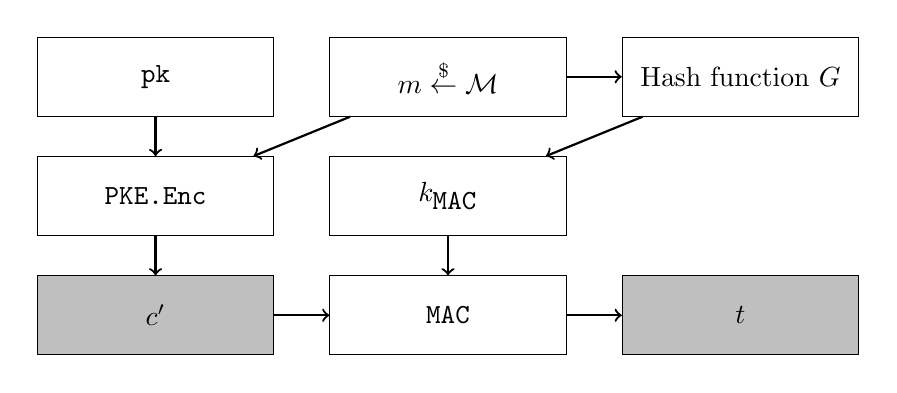
\begin{tikzpicture}
        \tikzstyle{rect} = [draw, rectangle, minimum width=3cm, minimum height=1cm]
        \tikzstyle{filledrect} = [draw, rectangle, minimum width=3cm, minimum height=1cm, fill=lightgray]
        \matrix [column sep=7mm, row sep=5mm] {
            \node (pk) [rect] {$\pk$}; &
            \node (m) [rect] {$m \leftsample \mathcal{M}$}; &
            \node (hashg) [rect] {Hash function $G$}; \\
            \node (pkeenc) [rect] {$\texttt{PKE.Enc}$}; &
            \node (mackey) [rect] {$k_\mac$}; \\
            \node (ct) [filledrect] {$c^\prime$}; &
            \node (mac) [rect] {$\mac$}; &
            \node (tag) [filledrect] {$t$}; \\
        };
        \draw[->, thick] (pk) -- (pkeenc);
        \draw[->, thick] (m) -- (pkeenc);
        \draw[->, thick] (m) -- (hashg);
        \draw[->, thick] (hashg) -- (mackey);
        \draw[->, thick] (pkeenc) -- (ct);
        \draw[->, thick] (mackey) -- (mac);
        \draw[->, thick] (ct) -- (mac);
        \draw[->, thick] (mac) -- (tag);
    \end{tikzpicture}

    \caption{Combining PKE with MAC using ``encrypt-then-MAC'' to encapsulate a shared secret. 
    The returned values are colored grey
    }\label{fig:etm-diagram}
\end{figure}

\subsubsection{Security reduction}
From a high level, the ``encrypt-then-MAC'' KEM encapsulates a shared secret by encrypting a randomly sampled PKE plaintext. To ensure the integrity of the ciphertext, a message authenticator is computed on the PKE ciphertext, where the symmetric key is derived by hashing the random PKE plaintext. The PKE ciphertext and message authenticator combine into the KEM ciphertext. For an adversary to produce a valid KEM ciphertext, it must produce a valid tag. If the message authenticator is existentially unforgeable, then the adversary cannot produce a valid tag without knowing the symmetric key, and under the random oracle model, this implies that the adversary must also know the corresonding PKE plaintext, thus rendering the decapsulation oracle's output redundant. 

We also extended the discussion of security requirement for the MAC: because each call to the encapsulation routine will use a freshly sampled PKE plaintext, each PKE ciphertext will be signed with a distinct MAC key. In other words, the MAC only needs to be one-time existentially unforgeable, which opens up possibilities of using more efficient constructions than HMAC and CBC-MAC as mentioned in the original paper.

In section \ref{sec:main-results}, we formally state the transformation and prove that the ``encrypt-then-MAC'' KEM is IND-CCA2 secure if the input PKE is OW-PCA secure and the input MAC is one-time existentially unforgeable.

\subsubsection{Performance improvements}
A major advantage of the ``encrypt-then-MAC'' construction is the low performance overhead added to the underlying PKE scheme. We instantiated the ``encrypt-then-MAC'' KEM with the underlying PKE routines of ML-KEM and compared its performance to ML-KEM, which uses the Fujisaki-Okamoto transformation. The Fujisaki-Okamoto transformation uses \emph{de-randomization} and \emph{re-encryption} to achieve chosen ciphertext security, which result in substantial performance penalty. When combined with the Poly1305 message authenticator, our construction $\text{ML-KEM}^+$ achieves on average 72\%-80\% reduction of CPU cycles needed for decapsulation while only incurring 2\%-7\% increase of CPU cycles for encapsulation when compared to ML-KEM.

\begin{table}[H]
    \centering
    \footnotesize

    \begin{tabular}{|p{1.2cm}|p{1.49cm}|p{1.49cm}|p{1.49cm}|p{1.49cm}|p{1.49cm}|p{1.49cm}|}
        \hline
        & ML-KEM \newline 512 & $\text{ML-KEM}^+$ \newline 512 
        & ML-KEM \newline 768 & $\text{ML-KEM}^+$ \newline 768 
        & ML-KEM \newline 1024 & $\text{ML-KEM}^+$ \newline 1024 
        \\
        \hline
        Encap \newline (ccl/tick) 
        & 91467 & 93157 \newline (+1.8\%) 
        & 136405 & 146405 \newline (+7.3\%) 
        & 199185 & 205763 \newline (+3.3\%) 
        \\
        \hline
        Decap \newline (ccl/tick) 
        & 121185 & 33733 \newline (-72.2\%) 
        & 186445 & 43315 \newline (-76.8\%) 
        & 246245 & 51375 \newline (-79.1\%) 
        \\
        \hline
        CT size \newline (bytes) 
        & 768 & 784 \newline (+2.1\%) 
        & 1088 & 1104 \newline (+1.5\%) 
        & 1568 & 1584 \newline (+1.0\%) 
        \\
        \hline
    \end{tabular}

    \caption{$\text{ML-KEM}^+$ is instantiated with Poly1305}
\end{table}

We also implemented and measured the round trip time of key exchange protocols with various modes of authentication. When compared to ML-KEM, $\text{ML-KEM}^+$ achieves 24\%-28\% reduction of round trip time in unauthenticated key exchange (KE), 29\%-35\% reduction in unilaterally authenticated key exchange (UAKE), and 35\%-48\% reduction in mutually authenticated key exchange (AKE).

\begin{table}[H]
    \centering
    \footnotesize

    \begin{tabular}{|p{1.6cm}|p{1.49cm}|p{1.49cm}|p{1.49cm}|p{1.49cm}|p{1.49cm}|p{1.49cm}|}
        \hline
        & ML-KEM \newline 512 & $\text{ML-KEM}^+$ \newline 512 
        & ML-KEM \newline 768 & $\text{ML-KEM}^+$ \newline 768 
        & ML-KEM \newline 1024 & $\text{ML-KEM}^+$ \newline 1024 
        \\
        \hline
        KE RTT \newline ($\us$) 
        & 92 & 70 \newline (-23.9\%) 
        & 135 & 99 \newline (-26.7\%) 
        & 193 & 138 \newline (-28.5\%) 
        \\
        \hline
        UAKE RTT \newline ($\us$) 
        & 145 & 103 \newline (-29.0\%) 
        & 215 & 144 \newline (-33.0\%) 
        & 310 & 202 \newline (-34.8\%) 
        \\
        \hline
        AKE RTT \newline ($\us$) 
        & 220 & 133 \newline (-39.5\%) 
        & 294 & 190 \newline (-35.4\%) 
        & 512 & 266 \newline (-48.0\%) 
        \\
        \hline
    \end{tabular}

    \caption{Key exchange round-trip times}
\end{table}

\subsection{Related works}
Optimal Asymmetric Encryption Padding (OAEP) \cite{bellare1995optimal}\cite{bellare1998relations} is a generic PKE construction whose IND-CCA2 security reduces to the one-wayness of the input trapdoor permutation under the random oracle model. OAEP enjoys tight security reduction and minimal performance overhead, but its requirement for a trapdoor permutation is difficult to satisfy. To this day, RSA remains the only practical candidate to instantiate OAEP with \cite{DBLP:journals/joc/Shoup02}\cite{DBLP:conf/crypto/FujisakiOPS01}, and RSA-OAEP saw widespread adoption in Internet communication protocols after its standardization in PKCS\#1 v2 \cite{rfc8017}.

Originally proposed by Eiichiro Fujisaki and Tatsuaki Okamoto, the Fujisaki-Okamoto transformation \cite{DBLP:conf/crypto/FujisakiO99}\cite{DBLP:journals/joc/FujisakiO13} is a hybid PKE whose security reduces non-tightly to the OW-CPA security of the input PKE. Later works by Hofheinz, Hovelmann, and Kiltz \cite{DBLP:conf/tcc/HofheinzHK17}\cite{DBLP:conf/asiacrypt/HovelmannsHM22} made systematic improvements to the original proposal by providing a modular KEM construction whose security tightly reduces to the IND-CPA security of the input PKE. In addition, the authors made extensive security analysis with respect to decryption failure (a non-trivial security flaws in many lattice-based cryptosystems) and provided a non-tight security reduction in the quantum random oracle model (QROM), which made the modular Fujisaki-Okamoto KEM suitable for post-quantum cryptography.

The modular Fujisaki-Okamoto KEM transformation is remarkably successful. It was adopted by many submissions to NIST's post-quantum cryptography competition, including Kyber \cite{DBLP:conf/eurosp/BosDKLLSSSS18}, Saber \cite{DBLP:conf/africacrypt/DAnversKRV18}, FrodoKEM \cite{DBLP:conf/ccs/BosCDMNNRS16}, and classic McEliece \cite{classicmceliecespec} among others. When Kyber was standardized by NIST in FIPS 203 ``Module-lattice key-encapsulation mechanism'' (ML-KEM) \cite{FIPS203}, it kept the Fujisaki-Okamoto transformation in its KEM construction. However, the Fujisaki-Okamoto transformation is not perfect. It uses \emph{de-randomization} and \emph{re-encryption} to achieve \emph{rigidity} \cite{bernstein2018towards} which then ensures ciphertext integrity. This brings two problems: \begin{itemize}
    \item \textbf{computational inefficiency:} where the PKE's encryption routine is substantially more expensive than the decryption routine, using re-encryption causes the decapsulation routine in the output KEM to become computationally expensive
    \item \textbf{side-channel vulnerability:} running the input PKE's encryption routine in the output KEM's decapsulation routine introduces risk of side-channel vulnerabilities not found in the input PKE's decryption routine alone. In fact, many practical attacks \cite{ueno2022curse}\cite{ravi2019generic} exploit re-encryption to decrypt ciphertext or recover secret keys. Countermeasures such as masking have been proposed to address these side channels, but they inevitably carry substantial performance penalty.
\end{itemize} 

% OAEP, REACT, GEM, 

\section{Preliminaries}

\subsection{Public-key encryption scheme}
\textbf{Syntax.} A public-key encryption scheme $\pke(\keygen, \encrypt, \decrypt)$ is a collection of three routines defined over some plaintext space $\mathcal{M}$ and some ciphertext space $\mathcal{C}$. $(\pk, \sk) \leftsample \keygen()$ is a randomized routine that returns a keypair. The encryption routine $\encrypt: (\pk, m) \mapsto c$ encrypts the input plaintext under the input public key. The decryption routine $\decrypt: (\sk, c) \mapsto m$ decrypts the input ciphertext under the input secret key. Where the encryption routine is randomized, we denote the randomness by $r \in \mathcal{R}$, where $\mathcal{R}$ is called the coin space. The decryption routine is assumed to always be deterministic. Some decryption routines can detect malformed ciphertext and output the rejection symbol $\bot$ accordingly.

\textbf{Correctness.} Following the definition in \cite{DBLP:conf/eurocrypt/DworkNR04} and \cite{hofheinz2017modular}, a $\pke$ is $\delta$-correct if:

\begin{equation*}
    E\left[\max_{m \in \mathcal{M}} P\left[\decrypt(\sk, c) \neq m \mid c \leftsample \encrypt(\pk, m)\right]\right] \leq \delta
\end{equation*}

Where the expectation is taken with respect to the probability distribution of all possible keypairs $(\pk, \sk) \leftsample \texttt{PKE.KeyGen()}$. For many lattice-based cryptosystems, including ML-KEM, decryption failures could leak information about the secret key, although the probability of a decryption failure is low enough that classical adversaries cannot exploit decryption failure more than they can defeat the underlying lattice problem. On the other hand, a quantum adversary may be able to exploit decryption failure in reasonable runtime by efficiently searching through all possible inputs using Grover's search algorithm. For that, ML-KEM made slight modifications in its KEM construction to prevent quantum adversary from precomputing large lookup table. We refer readers to \cite{avanzi2019crystals} and \cite{DBLP:conf/eurosp/BosDKLLSSSS18} for the details.

\textbf{Security.} We discuss the security of a $\pke$ using the sequence of games described in \cite{shoup2004sequences}. Specifically, we first define the $\texttt{OW-ATK}$ as they pertain to a public key encryption scheme. In later section we will define the $\texttt{IND-CCA}$ game as it pertains to a key encapsulation mechanism.

\def\algowatkgame{
    \begin{algorithm}[H]
        \caption*{The $\texttt{OW-ATK}$ game}
        \begin{algorithmic}[1]
            \State $(\pk, \sk) \leftsample \keygen(1^\lambda)$
            \State $m^\ast \leftsample \mathcal{M}$
            \State $c^\ast \leftsample \encrypt(\pk, m^\ast)$
            \State $\hat{m} \leftsample \mathcal{A}^{\mathcal{O}_\texttt{ATK}}(
                1^\lambda, \pk, c^\ast
            )$
            \State \Return $\llbrack m^\ast = \hat{m} \rrbrack$
        \end{algorithmic}
    \end{algorithm}
}
\def\algpco{
    \begin{algorithm}[H]
        \caption*{$\pco(m \in \mathcal{M}, c \in \mathcal{C})$}
        \begin{algorithmic}[1]
            \State \Return $\llbrack \decrypt(\sk, c) = m \rrbrack$
        \end{algorithmic}
    \end{algorithm}
}
\begin{figure}[H]
    \centering
    \begin{minipage}[b]{0.49\textwidth}
        \algowatkgame
    \end{minipage}
    \begin{minipage}[b]{0.49\textwidth}
        \algpco
    \end{minipage}
    \caption{
        One-way security game of PKE (left) and plaintext-checking oracle (right)
    }\label{fig:ow-game-pco}
\end{figure}

In the \texttt{OW-ATK} game (see figure \ref{fig:ow-game-pco}), an adversary's goal is to recover the decryption of a randomly generated ciphertext. A challenger randomly samples a keypair and a challenge plaintext $m^\ast$, encrypts the challenge plaintext $c^\ast \leftsample \encrypt(\pk, m^\ast)$, then gives $\pk$ and $c^\ast$ to the adversary $A$. The adversary $A$, with access to some oracle $\mathcal{O}_\texttt{ATK}$, outputs a guess decryption $\hat{m}$. $A$ wins the game if its guess $\hat{m}$ is equal to the challenge plaintext $m^\ast$. The \textit{advantage} $\adv_\texttt{OW-ATK}$ of an adversary in this game is the probability that it wins the game:

\begin{equation*}
    \adv_\texttt{OW-ATK}(A) = P\left[
        A(\pk, c^\ast) = m^\ast \vert
        (\pk, \sk) \leftsample \keygen() ;
        m^\ast \leftsample \mathcal{M};
        c^\ast \leftsample \encrypt(\pk, m^\ast)
    \right]
\end{equation*}

The capabilities of the oracle $\mathcal{O}_\texttt{ATK}$ depends on the choice of security goal $\texttt{ATK}$. Particularly relevant to our result is security against plaintext-checking attack (PCA), for which the adversary has access to a plaintext-checking oracle (PCO) (see figure \ref{fig:ow-game-pco}). A PCO takes as input a plaintext-ciphertext pair $(m, c)$ and returns \texttt{True} if $m$ is the decryption of $c$ or \texttt{False} otherwise.

\subsection{Key encapsulation mechanism (KEM)}
A key encapsulation mechanism is a collection of three routines $(\keygen, \encap, \decap)$ defined over some ciphertext space $\mathcal{C}$ and some key space $\mathcal{K}$. The key generation routine takes the security parameter $1^\lambda$ and outputs a keypair $(\pk, \sk) \leftsample \keygen(1^\lambda)$. $\encap(\pk)$ is a probabilistic routine that takes a public key $\pk$ and outputs a pair of values $(c, K)$ where $c \in \mathcal{C}$ is the ciphertext (also called encapsulation) and $K \in \mathcal{K}$ is the shared secret (also called session key). $\decap(\sk, c)$ is a deterministic routine that takes the secret key $\sk$ and the encapsulation $c$ and returns the shared secret $K$ if the ciphertext is valid. Some KEM constructions use explicit rejection, where if $c$ is invalid then $\decap$ will return a rejection symbol $\bot$; other KEM constructions use implicit rejection, where if $c$ is invalid then $\decap$ will return a fake session key that depends on the ciphertext and some other secret values.

The IND-CCA security of a KEM is defined by an adversarial game in which an adversary's goal is to distinguish pseudorandom shared secret (generated by running the $\encap$ routine) and a truly random value.

\begin{figure}[H]
    \centering
    \begin{minipage}[b]{0.49\textwidth}
        \begin{algorithm}[H]
            \caption*{KEM-IND-CCA2 game}
            \begin{algorithmic}[1]
                \State $(\pk, \sk) \leftsample \keygen(1^\lambda)$
                \State $(c^\ast, K_0) \leftsample \encap(\pk)$
                \State $K_1 \leftsample \mathcal{K}$
                \State $b \leftsample \{0, 1\}$
                \State $\hat{b} \leftsample A^{\mathcal{O}_\decap}(
                    1^\lambda, \pk, c^\ast, K_b
                )$
                \State \Return $\llbrack \hat{b} = b \rrbrack$
            \end{algorithmic}
        \end{algorithm}
    \end{minipage}\hfill
    \begin{minipage}[b]{0.49\textwidth}
        \begin{algorithm}[H]
        \caption*{$\mathcal{O}_\decap(c)$}
        \begin{algorithmic}[1]
            \State \Return $\decap(\sk, c)$
        \end{algorithmic}
        \end{algorithm}
    \end{minipage}
    \caption{IND-CCA2 game for KEM (left) and decapsulation oracle (right)}\label{fig:kem-game}
\end{figure}


The decapsulation oracle $\mathcal{O}^\decap$ takes a ciphertext $c$ and returns the output of the $\decap$ routine using the secret key. The advantage $\epsilon_\texttt{IND-CCA}$ of an IND-CCA adversary $\mathcal{A}_\texttt{IND-CCA}$ is defined by

\begin{equation*}
    \adv_\texttt{IND-CCA}(A) = \norm{
        P[A^{\mathcal{O}_\decap}(a^\lambda, \pk, c^\ast, K_b) = b] - \frac{1}{2}
    }
\end{equation*}

\subsection{Message authentication code (MAC)}\label{sec:message-authentication-code}
A message authentication code $\mac$ is a collection of routines $(\sign, \verify)$ defined over some key space $\mathcal{K}$, some message space $\mathcal{M}$, and some tag space $\mathcal{T}$. The signing routine $\sign(k, m)$ takes the secret key $k \in \mathcal{K}$ and some message, and outputs a tag $t$. The verification routine $\verify(k, m, t)$ takes the triplet of secret key, message, and tag, and outputs $\texttt{1}$ if the message-tag pair is valid under the secret key, or $\texttt{0}$ otherwise. Many MAC constructions are deterministic. For these constructions it is simpler to denote the signing routine by $t \leftarrow \mac(k, m)$ and perform verification using a simple comparison.

The security of a MAC is defined in an adversarial game in which an adversary, with access to some signing oracle $\mathcal{O}_\sign(m)$, tries to forge a new valid message-tag pair that has never been queried before. The existential unforgeability under chosen message attack (EUF-CMA) game is shown below:

\begin{figure}[H]
    \centering
    \begin{minipage}{0.7\textwidth}
        \begin{algorithm}[H]
            \caption*{\texttt{EUF-CMA} game}

            \begin{algorithmic}[1]
                \State $k^\ast \leftsample \mathcal{K}$
                \State $(\hat{m}, \hat{t}) \leftsample \mathcal{A}^{\mathcal{O}_\sign}()$
                \State \Return $
                    \llbrack \verify(k^\ast, \hat{m}, \hat{t}) 
                    \land (\hat{m}, \hat{t}) \not\in \mathcal{O}_\sign
                    \rrbrack
                $
            \end{algorithmic}
        \end{algorithm}
    \end{minipage}
    \caption{The existential forgery game}\label{fig:euf-cma-game}
\end{figure}

The advantage $\adv_\texttt{EUF-CMA}$ of the existential forgery adversary is the probability that it wins the EUF-CMA game.

\section{The ``encrypt-then-MAC'' transformation}\label{sec:main-results}
Let $\mathcal{B}^\ast$ denote the set of finite bit strings. Let $\pke(\keygen, \encrypt, \decrypt)$ be a public-key encryption scheme defined over message space $\mathcal{M}$ and ciphertext space $\mathcal{C}$. Let $\mac: \mathcal{K}_\mac \times \mathcal{B}^\ast \rightarrow \mathcal{T}$ be a deterministic message authentication code that takes a key $k \in \mathcal{K}_\mac$, some message $m \in \mathcal{B}^\ast$, and outputs a digest $t \in \mathcal{T}$. Let $G: \mathcal{M} \rightarrow \mathcal{K}_\mac$ be a hash function that maps from $\pke$'s plaintext space to $\mac$'s key space. Let $H: \mathcal{B}^\ast \rightarrow \mathcal{K}_\kem$ be a hash function that maps bit strings into the set of possible shared secrets. The ``encrypt-then-MAC'' transformation $\etm[\pke, \mac, G, H]$ constructs a key encapsulation mechanism $\kem_\etm(\keygen_\kem, \encap, \decap)$, whose routines are described in figure \ref{fig:etm-routines}.

\begin{figure}[H]
    \centering
    \begin{minipage}[t]{0.5\textwidth}
        \begin{algorithm}[H]
            \caption*{$\kem_\etm.\keygen()$}
            \begin{algorithmic}[1]
                \State $(\pk, \sk^\prime) \leftsample \pke\texttt{.}\keygen()$
                \State $z \leftsample \mathcal{M}$
                \State $\sk \leftarrow \sk^\prime \Vert z$
                \State \Return $(\pk, \sk)$
            \end{algorithmic}
        \end{algorithm}
        \begin{algorithm}[H]
            \caption*{$\kem_\etm.\encap(\pk)$}
            \begin{algorithmic}[1]
                \State $m \leftsample \mathcal{M}$
                \State $k \leftarrow G(m)$
                \State $c^\prime \leftsample \pke\texttt{.}\encrypt(\pk, m)$
                \State $t \leftarrow \mac(k, c^\prime)$
                \State $K \leftarrow H(m, c^\prime)$
                \State $c \leftarrow c^\prime \Vert t$
                \State \Return $(c, K)$
            \end{algorithmic}
        \end{algorithm}
    \end{minipage}\hfill
    \begin{minipage}[t]{0.49\textwidth}
        \begin{algorithm}[H]
            \caption*{$\kem_\etm.\decap(\sk, c)$}
            \begin{algorithmic}[1]
                \State $(c^\prime, t) \leftarrow c$
                \State $(\sk^\prime, z) \leftarrow \sk$
                \State $\hat{m} \leftarrow \pke\texttt{.}\decrypt(\sk^\prime, c^\prime)$
                \State $\hat{k} \leftarrow G(\hat{m})$
                \If{$\mac(\hat{k}, c^\prime) \neq t$}
                    \State $K \leftarrow H(z, c^\prime)$
                \Else
                    \State $K \leftarrow H(\hat{m}, c^\prime)$
                \EndIf
                \State \Return $K$
            \end{algorithmic}
        \end{algorithm}
    \end{minipage}
    \caption{$\kem_\etm$ routines}\label{fig:etm-routines} 
\end{figure}

The key generation routine of $\kem_\etm$ is largely identical to that of the $\pke$, only a secret value $z$ is sampled as the implicit rejection symbol. In the encapsulation routine, a MAC key is derived from the randomly sampled plaintext $k \leftarrow G(m)$, then used to sign the unauthenticated ciphertext $c^\prime$. Because the encryption routine might be randomized, the session key is derived from both the message and the ciphertext. Finally, the unauthenticated ciphertext $c^\prime$ and the tag $t$ combine into the authenticated ciphertext $c$ that would be transmitted to the peer. In the decapsulation routine, the decryption $\hat{m}$ of the unauthenticated ciphertext is used to re-derive the MAC key $\hat{k}$, which is then used to re-compute the tag $\hat{t}$. The ciphertext is considered valid if and only if the recomputed tag is identical to the input tag.

For an adversary $A$ to produce a valid tag $t$ for some unauthenticated ciphertext $c^\prime$ under the symmetric key $k \leftarrow G(\decrypt(\sk^\prime, c^\prime))$ implies that $A$ must either know the symmetric key $k$ or produce a forgery. Under the random oracle model, $A$ also cannot know $k$ without knowing its preimage $\decrypt(\sk^\prime, c^\prime)$, so $A$ must either have produced $c^\prime$ honestly, or have broken the one-way security of $\pke$. This means that the decapsulation oracle will not give out information on decryptions that the adversary does not already know. 

\begin{figure}[H]
    \centering
    \begin{minipage}{0.6\textwidth}
    \begin{algorithm}[H]
        \caption*{$\pco(m, c)$}
        \begin{algorithmic}[1]
            \State $k \leftarrow G(m)$
            \State $t \leftarrow \mac(k, c)$
            \State \Return $\llbrack \mathcal{O}^\decap((c, t)) = H(m, c)\rrbrack$
        \end{algorithmic}
    \end{algorithm}
    \end{minipage}
    \caption{Every decapsulation oracle can be converted into a plaintext-checking oracle}\label{fig:pco-using-decap-oracle}
\end{figure}

However, a decapsulation oracle can still give out some information: for a known plaintext $m$, all possible encryptions $c^\prime \leftsample \encrypt(\pk, m)$ can be correctly signed, while ciphertexts that don't decrypt back to $m$ cannot be correctly signed. This means that a decapsulation oracle can be converted into a plaintext-checking oracle (see figure \ref{fig:pco-using-decap-oracle}), so every chosen-ciphertext attack against the KEM can be converted into a plaintext-checking attack against the underlying PKE.

On the other hand, if the underlying PKE is one-way secure against plaintext-checking attack that makes $q$ plaintext-checking queries, then ``encrypt-then-MAC'' KEM is semantically secure under chosen ciphertext attacks making the same number of decapsulation queries:

\begin{theorem}\label{thm:ow-pca-implies-kem-ind-cca2}
    For every \texttt{IND-CCA2} adversary $A$ against $\kem_\etm$ that makes $q$ decapsulation queries, there exists an \texttt{OW-PCA} adversary $B$ who makes at least $q$ plaintext-checking queries against the underlying $\pke$, and an one-time existential forgery adversary $C$ against the underlying $\mac$ such that

    \begin{equation*}
        \texttt{Adv}_\texttt{IND-CCA2}(A) \leq q \cdot \adv_\texttt{OT-MAC}(C) + 2 \cdot \texttt{Adv}_\texttt{OW-PCA}(B)
    \end{equation*}
\end{theorem}

Theorem \ref{thm:ow-pca-implies-kem-ind-cca2} naturally flows into an equivalence relationship between the security of the KEM and the security of the PKE:

\begin{lemma}
    $\kem_\etm$ is IND-CCA2 secure if and only if the input $\pke$ is OW-PCA secure
\end{lemma}

\subsection{Proof of theorem \ref{thm:ow-pca-implies-kem-ind-cca2}}
We will prove theorem \ref{thm:ow-pca-implies-kem-ind-cca2} using a sequence of game. A summary of the the sequence of games can be found in figure \ref{fig:etm-ind-cc2-sequence-of-games} and \ref{fig:ow-pca-simulates-game-3}. From a high level we made three incremental modifications to the IND-CCA2 game for $\kem_\etm$: replace true decapsulation with simulated decapsulation, replace the pseudorandom MAC key $k^\ast \leftarrow G(m^\ast)$ with a truly random MAC key $k^\ast \leftsample \mathcal{K}_\mac$, and finally replace pseudorandom shared secret $K_0 \leftarrow H(m^\ast, c^\prime)$ with a truly random shared secret $K_0 \leftsample \mathcal{K}_\kem$. A OW-PCA adversary can then simulate the modified IND-CCA2 game for the KEM adversary, and the advantage of the OW-PCA adversary is associated with the probability of certain behaviors of the KEM adversary.

\begin{figure}[h]
    \centering
    \begin{minipage}[t]{0.5\textwidth}
        \begin{algorithm}[H]
            \caption*{\texttt{IND-CCA2} game for $\kem_\etm$}
            \begin{algorithmic}[1]
                \State $(\pk, \sk) \leftsample \kem_\etm\texttt{.}\keygen()$
                \State $m^\ast \leftsample \mathcal{M}$
                \State $c^\prime \leftsample \pke\texttt{.}\encrypt(\pk, m^\ast)$
                \State $k^\ast \leftarrow G(m^\ast)$
                    \Comment{Game 0-1}
                \State $k^\ast \leftsample \mathcal{K}_\mac$
                    \Comment{Game 2-3}
                \State $t \leftarrow \mac(k^\ast, c^\prime)$
                \State $c^\ast \leftarrow c^\prime \Vert t$
                \State $K_0 \leftarrow H(m^\ast, c^\prime)$
                    \Comment{Game 0-2}
                \State $K_0 \leftsample \mathcal{K}_\kem$
                    \Comment{Game 3}
                \State $K_1 \leftsample \mathcal{K}_\kem$
                \State $b \leftsample \{0,1\}$
                \State $\hat{b} \leftarrow A^{\mathcal{O}^\decap}(\pk, c^\ast, K_b)$
                    \Comment{Game 0}
                \State $\hat{b} \leftarrow A^{\mathcal{O}^\decap_1}(\pk, c^\ast, K_b)$
                    \Comment{Game 1-3}
                \State \Return $\llbrack \hat{b} = b \rrbrack$
            \end{algorithmic}
        \end{algorithm}
        \begin{algorithm}[H]
            \caption*{$\mathcal{O}^G(m)$}
            \begin{algorithmic}[1]
                \If{$\exists (\tilde{m}, \tilde{k}) \in \mathcal{L}^G : \tilde{m} = m$}
                    \State \Return $\tilde{k}$
                \EndIf
                \State $k \leftsample \mathcal{K}_\mac$
                \State $\mathcal{L}^G \leftarrow \mathcal{L}^G \cup \{(m, k)\}$
                \State \Return $k$
            \end{algorithmic}
        \end{algorithm}
    \end{minipage}
    \begin{minipage}[t]{0.49\textwidth}
        \begin{algorithm}[H]
            \caption*{$\mathcal{O}^\decap(c)$}
            \begin{algorithmic}[1]
                \State $(c^\prime, t) \leftarrow c$
                \State $\hat{m} = \decrypt(\sk^\prime, c^\prime)$
                \State $\hat{k} \leftarrow G(\hat{m})$
                \If{$\mac(\hat{k}, c^\prime) = t$}
                    \State $K \leftarrow H(\hat{m}, c^\prime)$
                \Else 
                    \State $K \leftarrow H(z, c^\prime)$
                \EndIf 
                \State \Return $K$
            \end{algorithmic}
        \end{algorithm}
        \vspace{-0.5cm}
        \begin{algorithm}[H]
            \caption*{$\mathcal{O}^\decap_1(c)$}
            \begin{algorithmic}[1]
                \State $(c^\prime, t) \leftarrow c$
                \If{$\exists (\tilde{m}, \tilde{k}) \in \mathcal{L}^G : 
                    \tilde{m} = \decrypt(\sk^\prime, c^\prime)
                    \land \mac(\tilde{k}, c^\prime) = t
                $}
                    \State $K \leftarrow H(\tilde{m}, c^\prime)$
                \Else
                    \State $K \leftarrow H(z, c^\prime)$
                \EndIf
                \State \Return $K$
            \end{algorithmic}
        \end{algorithm}
        \vspace{-0.5cm}
        \begin{algorithm}[H]
            \caption*{$\mathcal{O}^H(m, c)$}
            \begin{algorithmic}[1]
                \If{$\exists (\tilde{m}, \tilde{c}, \tilde{K}) \in \mathcal{L}^H : \tilde{m} = m \land \tilde{c} = c$}
                    \State \Return $\tilde{K}$
                \EndIf
                \State $K \leftsample \mathcal{K}_\kem$
                \State $\mathcal{L}^H \leftarrow \mathcal{L}^H \cup \{(m, c, K)\}$
                \State \Return $K$
            \end{algorithmic}
        \end{algorithm}
    \end{minipage}
    \caption{Sequence of games}\label{fig:etm-ind-cc2-sequence-of-games}
\end{figure}

\begin{proof}
    \emph{Game 0} is the standard IND-CCA2 game for KEMs. The decapsulation oracle $\mathcal{O}^\decap$ executes the decapsulation routine using the challenge keypair and return the results faithfully. The queries made to the hash oracles $\mathcal{O}^G, \mathcal{O}^H$ are recorded to their respective tapes $\mathcal{L}^G, \mathcal{L}^H$.

    \emph{Game 1} is identical to game 0 except that the true decapsulation oracle $\mathcal{O}^\decap$ is replaced with a simulated oracle $\mathcal{O}^\decap_1$. Instead of directly decrypting $c^\prime$ as in the decapsulation routine, the simulated oracle searches through the tape $\mathcal{L}^G$ to find a matching query $(\tilde{m}, \tilde{k})$ such that $\tilde{m}$ is the decryption of $c^\prime$. The simulated oracle then uses $\tilde{k}$ to validate the tag $t$ against $c^\prime$.

    If the simulated oracle accepts the queried ciphertext as valid, then there is a matching query that also validates the tag, which means that the queried ciphertext is honestly generated. Therefore, the true oracle must also accept the queried ciphertext. On the other hand, if the true oracle rejects the queried ciphertext (and output the implicit rejection $H(z, c^\prime)$), then the tag is simply invalid under the MAC key $k = G(\decrypt(\sk^\prime, c^\prime))$. Therefore, there could not have been a matching query that also validates the tag, and the simulated oracle must also rejects the queried ciphertext.

    This means that from the adversary $A$'s perspective, game 1 and game 0 differ only when the true oracle accepts while the simulated oracle rejects, which means that $t$ is a valid tag for $c^\prime$ under $k = G(\decrypt(\sk^\prime, c^\prime))$, but $k$ has never been queried. Under the random oracle model, such $k$ is a uniformly random sample of $\mathcal{K}_\mac$ that the adversary does not know, so for $A$ to produce a valid tag is to produce a forgery against the $\mac$ under an unknown and uniformly random key. Furthermore, the security game does not include a signing oracle, so this is a zero-time forgery. While zero-time forgery is not a standard security definition for a MAC, we can bound it by the advantage of a one-time forgery adversary $C$:

    \begin{equation*}
        P\left[\mathcal{O}^\decap(c) \neq \mathcal{O}^\decap_1(c)\right]
        \leq \adv_\texttt{OT-MAC}(C)
    \end{equation*}

    Across all $q$ decapsulation queries, the probability that at least one query is a forgery is thus at most $q \cdot P\left[\mathcal{O}^\decap(c) \neq \mathcal{O}^\decap_1(c)\right]$. By the difference lemma:

    \begin{equation*}
        \adv_{G_0}(A) - \adv_{G_1}(A) \leq q\cdot  \adv_\texttt{OT-MAC}(C)
    \end{equation*}

    \emph{Game 2} is identical to game 1, except that the challenger samples a uniformly random MAC key $k^\ast \leftsample \mathcal{K}_\mac$ instead of deriving it from $m^\ast$. From $A$'s perspective the two games are indistinguishable, unless $A$ queries $G$ with the value of $m^\ast$. Denote the probability that $A$ queries $G$ with $m^\ast$ by $P[\texttt{QUERY G}]$, then:

    \begin{equation*}
        \adv_{G_1}(A) - \adv_{G_2}(A) \leq P\left[\texttt{QUERY G}\right]
    \end{equation*}

    \emph{Game 3} is identical to game 2, except that the challenger samples a uniformly random shared secret $K_0 \leftsample \mathcal{K}_\kem$ instead of deriving it from $m^\ast$ and $c^\prime$. From $A$'s perspective the two games are indistinguishable, unless $A$ queries $H$ with $(m^\ast, \cdot)$. Denote the probability that $A$ queries $H$ with $(m^\ast, \cdot)$ by $P[\texttt{QUERY H}]$, then:

    \begin{equation*}
        \adv_{G_2}(A) - \adv_{G_3}(A) \leq P\left[\texttt{QUERY H}\right]
    \end{equation*}

    Since in game 3, both $K_0$ and $K_1$ are uniformly random and independent of all other variables, no adversary can have any advantage: $\adv_{G_3}(A) = 0$.

    \begin{figure}[h]
        \begin{minipage}[t]{0.49\textwidth}
            \begin{algorithm}[H]
                \caption*{$B(\pk, {c^\prime}^\ast)$}
                \begin{algorithmic}[1]
                    \State $z \leftsample \mathcal{M}$
                    \State $k \leftsample \mathcal{K}_\mac$
                    \State $t \leftarrow \mac(k, {c^\prime}^\ast)$
                    \State $c^\ast \leftarrow ({c^\prime}^\ast, t)$
                    \State $K \leftsample \mathcal{K}_\kem$
                    \State $\hat{b} \leftarrow A^{
                        \mathcal{O}^\decap_B, \mathcal{O}^G_B, \mathcal{O}^H_B
                    }(\pk, c^\ast, K)$
                    \If{$\texttt{ABORT}(m)$}
                        \State \Return $m$
                    \EndIf
                \end{algorithmic}
            \end{algorithm}
            \begin{algorithm}[H]
                \caption*{$\mathcal{O}^H_B(m, c)$}
                \begin{algorithmic}
                    \If{$\pco(m, {c^\prime}^\ast) = 1$}
                        \State $\texttt{ABORT}(m)$
                    \EndIf
                    \If{$
                        \exists (\tilde{m}, \tilde{c}, \tilde{K}) \in \mathcal{L}^H 
                        : \tilde{m} = m \land \tilde{c} = c
                    $}
                        \State \Return $\tilde{K}$
                    \EndIf
                    \State $K \leftsample \mathcal{K}_\kem$
                    \State $\mathcal{L}^H \leftarrow \mathcal{L}^H \cup \{(m, c, K)\}$
                    \State \Return $K$
                \end{algorithmic}
            \end{algorithm}
        \end{minipage}\hfill
        \begin{minipage}[t]{0.49\textwidth}
            \begin{algorithm}[H]
                \caption*{$\mathcal{O}^\decap_B(c)$}
                \begin{algorithmic}[1]
                    \State $(c^\prime, t) \leftarrow c$
                    \If{$\exists (\tilde{m}, \tilde{k}) \in \mathcal{L}^G : 
                        % \tilde{m} = \decrypt(\sk^\prime, c^\prime)
                        \pco(c^\prime, \tilde{m}) = 1
                        \land \mac(\tilde{k}, c^\prime) = t
                    $}
                        \State $K \leftarrow H(\tilde{m}, c^\prime)$
                    \Else
                        \State $K \leftarrow H(z, c^\prime)$
                    \EndIf
                    \State \Return $K$
                \end{algorithmic}
            \end{algorithm}
            \begin{algorithm}[H]
                \caption*{$\mathcal{O}^G_B(m)$}
                \begin{algorithmic}[1]
                    \If{$\pco(m, {c^\prime}^\ast) = 1$}
                        \State $\texttt{ABORT}(m)$
                    \EndIf
                    \If{$\exists (\tilde{m}, \tilde{k}) \in \mathcal{L}^G : \tilde{m} = m$}
                        \State \Return $\tilde{k}$
                    \EndIf
                    \State $k \leftsample \mathcal{K}_\mac$
                    \State $\mathcal{L}^G \leftarrow \mathcal{L}^G \cup \{(m, k)\}$
                    \State \Return $k$
                \end{algorithmic}
            \end{algorithm}
        \end{minipage}
        \caption{OW-PCA adversary $B$ simulates game 3 for IND-CCA2 adversary $A$}\label{fig:ow-pca-simulates-game-3}
    \end{figure}

    We will bound $P[\texttt{QUERY G}]$ and $P[\texttt{QUERY H}]$ by constructing a OW-PCA adversary $B$ against the underlying PKE that uses $A$ as a sub-routine. $B$'s behaviors are summarized in figure \ref{fig:ow-pca-simulates-game-3}.

    $B$ simulates game 3 for $A$: receiving the public key $\pk$ and challenge encryption ${c^\prime}^\ast$, $B$ samples random MAC key and session key to produce the challenge encapsulation, then feeds it to $A$. When simulating the decapsulation oracle, $B$ uses the plaintext-checking oracle to look for matching queries in $\mathcal{L}^G$. When simulating the hash oracles, $B$ uses the plaintext-checking oracle to detect when $m^\ast = \decrypt(\sk^\prime, {c^\prime}^\star)$ has been queried. When $m^\ast$ is queried, $B$ terminates $A$ and returns $m^\ast$ to win the OW-PCA game. In other words:

    \begin{equation*}
        \begin{aligned}
            P\left[\texttt{QUERY G}\right] &\leq \adv_\texttt{OW-PCA}(B) \\
            P\left[\texttt{QUERY H}\right] &\leq \adv_\texttt{OW-PCA}(B) \\
        \end{aligned}
    \end{equation*}

    Combining all equations above produce the desired security bound.
\end{proof}

\section{Implementation}\label{sec:implementation}
ML-KEM is an \texttt{IND-CCA2} secure key encapsulation mechanism standardized by NIST in FIPS 203. The \texttt{IND-CCA2} security of ML-KEM is achieved in two steps. First, ML-KEM constructs an \texttt{IND-CPA} secure public key encryption scheme $\texttt{K-PKE}(\keygen, \encrypt, \decrypt)$ whose security is based on the conjectured intractability of the module learning with error (MLWE) problems against both classical and quantum adversaries. Then, the $U^{\not\bot}_m$ variant of the Fujisaki-Okamoto transformation \cite{hofheinz2017modular} is used to construct the KEM $\texttt{MLKEM}(\keygen, \encap, \decap)$ by calling $\texttt{K-PKE}(\keygen, \encrypt, \decrypt)$ as sub-routines. Because $\texttt{K-PKE}.\encrypt$ includes substantially more arithmetics than $\texttt{K-PKE}.\decrypt$, by using \textit{re-encryption} and \textit{de-randomization}, ML-KEM's decapsulation routine incurs significant computational cost. 

We implemented the ``encrypt-then-MAC'' KEM construction using $\texttt{K-PKE}$ as the input PKE and compared its performance against ML-KEM under a variety of scenarios. The experimental data showed that while the ``encrypt-then-MAC'' construction adds a small amount of computational overhead to the encapsulation routine and a small increase in ciphertext size when compared with ML-KEM, it boasts enormous runtime savings in the decapsulation routine, which makes it particularly suitable for deployment in constrained environment. See appendix \ref{sec:ml-kem-and-kyber} for comparison with Kyber's third round submission to NIST's PQC competition.

We refer readers to \cite{FIPS203} for the details of the \texttt{K-PKE} routines. The ``encrypt-then-MAC'' KEM routines are described in figure \ref{fig:ml-kem-plus-routines} below.

\begin{figure}[H]
    \centering

    \begin{minipage}[t]{0.5\textwidth}
        \begin{algorithm}[H]
            \caption*{$\texttt{ML-KEM}^\texttt{+}\texttt{.}\keygen\texttt{()}$}
            \begin{algorithmic}[1]
                \State $z \leftsample \{0,1\}^{256}$
                \State $(\pk, \sk^\prime) \leftsample \texttt{K-PKE}.\keygen()$
                \State $h \leftarrow H(\pk)$
                \State $\sk \leftarrow (sk^\prime \Vert \pk \Vert h \Vert z)$
                \State \Return $(\pk, \sk)$
            \end{algorithmic}
        \end{algorithm}\vspace{-0.5cm}
        \begin{algorithm}[H]
            \caption*{$\texttt{ML-KEM}^\texttt{+}\texttt{.}\encap\texttt{(\pk)}$}
            \begin{algorithmic}[1]
                \Require Public key $\pk$
                \State $m \leftsample \{0,1\}^{256}$
                \State $(\overline{K}, r, k) \leftarrow \texttt{XOF}(m \Vert H(\pk))$
                \State $c^\prime \leftarrow \texttt{K-PKE}.\encrypt(\pk, m, r)$
                \State $t \leftarrow \mac(k, c^\prime)$
                \State $K \leftarrow \texttt{KDF}(\overline{K} \Vert c^\prime)$
                \State $c \leftarrow (c^\prime, t)$
                \State \Return $(c, K)$
            \end{algorithmic}
        \end{algorithm}
    \end{minipage}\hfill
    \begin{minipage}[t]{0.49\textwidth}
        \begin{algorithm}[H]
            \caption*{$\texttt{ML-KEM}^\texttt{+}\texttt{.}\decap\texttt{(\sk, c)}$}
            \begin{algorithmic}[1]
                \Require Secret key $\sk = (\sk^\prime \Vert \pk \Vert h \Vert z)$
                \Require Ciphertext $c = (c^\prime \Vert t)$
                \State $(\sk^\prime, \pk, h, z) \leftarrow \sk$
                \State $(c^\prime, t) \leftarrow c$
                \State $\hat{m} \leftarrow \texttt{K-PKE}.\decrypt(\sk^\prime, c^\prime)$
                \State $(\overline{K}, \hat{r}, \hat{k}) \leftarrow \texttt{XOF}(\hat{m} \Vert h)$
                \State $\hat{t} \leftarrow \mac(\hat{k}, c^\prime)$
                \If{$\hat{t} = t$}
                    \State $K \leftarrow \texttt{KDF}(\overline{K} \Vert t)$
                \Else
                    \State $K \leftarrow \texttt{KDF}(z \Vert t)$
                \EndIf
                \State \Return $K$
            \end{algorithmic}
        \end{algorithm}
    \end{minipage}

    \caption{$\texttt{ML-KEM}^+$ routines}\label{fig:ml-kem-plus-routines}
\end{figure}

Our implementation extended from the reference implementation by the PQCrystals team (https://github.com/pq-crystals/kyber). All C code is compiled with \texttt{GCC 11.4.1} and \texttt{OpenSSL 3.0.8}. All binaries are executed on an AWS c7a.medium instance with an AMD EPYC 9R14 CPU at 3.7 GHz and 1 GB of RAM.

\subsection{Choosing a message authenticator}
For the $\texttt{ML-KEM}^+$ implementation, we instantiated $\mac$ with a selection that covered a wide range of MAC designs, including Poly1305 \cite{bernstein2005poly1305}, GMAC \cite{mcgrew2004galois}, CMAC \cite{iwata2003omac}\cite{black2000cbc}, and KMAC \cite{SP80053r4}.

Poly1305 and GMAC are both Carter-Wegman style authenticators \cite{wegman1981new} that compute the tag using finite field arithmetic. Generically speaking, Carter-Wegman MAC is parameterized by some finite field $\mathbb{F}$ and the maximal message length $L > 0$. Each symmetric key $k = (k_1, k_2) \leftsample \mathbb{F}^2$ is a pair of uniformly ranodm field elements, and the message is parsed into tuples of field elements up to length $L$: $m = (m_1, m_2, \ldots, m_l) \in \mathbb{F}^{\leq L}$. The tag $t$ is computed by evaluating a polynomial whose coefficients the message blocks and whose indeterminate is the key:

\begin{equation}\label{eq:carter-wegman-one-time-mac}
    \mac((k_1, k_2), m) = H_\text{xpoly}(k_1, m) + k_2
\end{equation}

Where $H_\text{xpoly}$ is given by:

\begin{equation*}
    H_\text{xpoly}(k_1, m) = k_1^{l+1} + k_1^l \cdot m_1 + k_1^{l-1} \cdot m_2 + \ldots + k_1 \cdot m_l
\end{equation*}

The authenticator formulated in equation \ref{eq:carter-wegman-one-time-mac} is a one-time MAC. To make the construction many-time secure, a non-repeating nonce $r$ and a PRF is needed:

\begin{equation*}
    \mac((k_1, k_2), m, r) = H_\text{xpoly}(k_1, m) \oplus \texttt{PRF}(k_2, r)
\end{equation*}

Specifically, Poly1035 operates in the prime field $\mathbb{F}_q$ where $q = 2^{130} - 5$ whereas GMAC operates in the binary field $\mathbb{F}_{2^{128}}$. In OpenSSL's implementation, standalone Poly1305 is a one-time secure MAC, whereas GMAC uses a nonce and AES as the PRF and is thus many-time secure (in OpenSSL GMAC is AES-256-GCM except all data is fed into the ``associated data'' section and thus not encrypted).

CMAC is based on the CBC-MAC with the block cipher instantiated from AES-256. To compute a CMAC tag, the message is first broke into 128-bit blocks with appropriate padding. Each block is first XOR'd with the previous block's output, then encrypted under AES using the symmetric key. The final output is XOR'd with a sub key derived from the symmetric key, before being encrypted for one last time. %A summary of the computation can be found in figure \ref{fig:aes-256-cmac}

% \begin{figure}[h]
%     \centering
%     \begin{minipage}[t]{0.49\textwidth}
%         \begin{algorithm}[H]
%             \caption*{Sub-key derivation}
%             \begin{algorithmic}[1]
%                 \Require 256-bit key $k$
%                 \Require $\texttt{const\_Rb = 0x87}$
%                 \State $l \leftarrow \texttt{AES-256}(k, 0^{128})$
%                 \If{$\texttt{MostSignificantBit}(l) = 0$}
%                     \State $k_1 \leftarrow \texttt{l {<}{<} 1}$
%                 \Else 
%                     \State $k_1 \leftarrow \texttt{l {<}{<} 1} \oplus \texttt{const\_Rb}$
%                 \EndIf
%                 \If{$\texttt{MostSignificantBit}(k_1) = 0$}
%                     \State $k_2 \leftarrow k_1 \texttt{ {<}{<} 1}$
%                 \Else 
%                     \State $k_2 \leftarrow k_1 \texttt{ {<}{<} 1} \oplus \texttt{const\_Rb}$
%                 \EndIf
%                 \State \Return $k_1, k_2$
%             \end{algorithmic}
%         \end{algorithm}
%     \end{minipage}\hfill
%     \begin{minipage}[t]{0.49\textwidth}
%         \begin{algorithm}[H]
%             \caption*{CMAC(k, m)}
%             \begin{algorithmic}[1]
%                 \Require 256-bit symmetric key $k$
%                 \State $(k_1, k_2) \leftarrow \texttt{deriveSubKey}(k)$
%                 \State $n \leftarrow \left\lceil \texttt{bytesLen}(m) / 16\right\rceil$
%                 \If{$n = 0$}
%                     \State $n \leftarrow 1$
%                     \State $m_\texttt{last} \leftarrow m_n \oplus k_2$
%                 \ElsIf{$\texttt{bytesLen(m)} \mod 16 = 0$}
%                     \State $m_\texttt{last} \leftarrow m_n \oplus k_1$
%                 \Else 
%                     \State $m_\texttt{last} \leftarrow m_n \oplus k_2$
%                 \EndIf

%                 \State $x = 0^{128}$
%                 \For{$i \in \{1, 2, \ldots, n-1\}$}
%                     \State $y \leftarrow x \oplus m_i$
%                     \State $x \leftarrow \texttt{AES-256}(k, y)$
%                 \EndFor
%                 \State $y \leftarrow m_\texttt{last} \oplus x$
%                 \State $t \leftarrow \texttt{AES-256}(k, y)$
%                 \State \Return $t$
%             \end{algorithmic}
%         \end{algorithm}
%     \end{minipage}
%     \caption{AES-256 CMAC}\label{fig:aes-256-cmac}
% \end{figure}

KMAC is defined in \cite{SP80053r4} to be based on the family of sponge functions with Keccak permutaiton as the underlying function. We chose KMAC-256, which uses Shake256 as the underlying extendable output functions. KMAC allows variable-length key and tag, but we chose the 256 bits for key length and 128 bits for tag size for consistency with other authenticators.

To isolate the performance characteristics of each authenticator in our instantiation of $\texttt{ML-KEM}^+$, we measured the CPU cycles needed for each authenticator to compute a tag on random inputs whose sizes correspond to the ciphertext sizes of \texttt{ML-KEM}. The measurements are summarized in table \ref{tbl:mac-performance}.

From our testing, we found Poly1305 to exhibit the best performance characteristics. However, there are additional security considerations that may require the use of other less efficient MAC instances. For example, it is possible for an adversary with large computing infrastructure or quantum computers to pre-compute a large lookup table mapping symmetric key to the source plaintext. Upon receiving a ciphertext, the adversary can then search through the lookup table for a matching key, which would've revealed the corresponding decryption. We partially mitigated such attack by deriving the symmetric key from both the public key and the plaintext, but in case of a long-term keypair, the adversary might still be able to compute a large lookup table AFTER obtaining the long-term public key. Further mitigation could include using larger-size keys, which can be accomplished either by using a Carter-Wegman MAC that operates on a larger finite field or using a MAC with a variable key-length such as KMAC.

\begin{table}[H]
    \centering
    \footnotesize
    \caption{CPU cycles needed to compute tag on various input sizes}\label{tbl:mac-performance}
    \begin{tabular}{|c|c|c|}
        \hline
        \multicolumn{3}{|c|}{\bf Input size: 768 bytes} \\
        \hline
        MAC & Median & Average \\
        \hline
        Poly1305 & 909 & 2823 \\
        \hline
        GMAC & 3899 & 4859 \\
        \hline
        CMAC & 6291 & 6373 \\
        \hline
        KMAC & 6373 & 7791 \\
        \hline
    \end{tabular}
    \begin{tabular}{|c|c|c|}
        \hline
        \multicolumn{3}{|c|}{\bf Input size: 1088 bytes} \\
        \hline
        MAC & Median & Average \\
        \hline
        Poly1305 & 961 & 2704 \\
        \hline
        GMAC & 3899 & 4827 \\
        \hline
        CMAC & 7305 & 7588 \\
        \hline
        KMAC & 9697 & 9928 \\
        \hline
    \end{tabular}
    \begin{tabular}{|c|c|c|}
        \hline
        \multicolumn{3}{|c|}{\bf Input size: 1568 bytes} \\
        \hline
        MAC & Median & Average \\
        \hline
        Poly1305 & 1065 & 1809 \\
        \hline
        GMAC & 4055 & 5026 \\
        \hline
        CMAC & 8735 & 8772 \\
        \hline
        KMAC & 11647 & 12186 \\
        \hline
    \end{tabular}
\end{table}

\subsection{KEM performance}
Compared to the $U^{\not\bot}_m$ variant of Fujisaki-Okamoto transformed used in ML-KEM, the ``encrypt-then-MAC'' transformation the following trade-off when given the same input sub-routines: \begin{enumerate}
    \item Both encapsulation and decapsulation add a small amount of overhead for needing to hash both the PKE plaintext and the PKE ciphertext when deriving the shared secret, where as the $U^{\not\bot}_m$ transformation only needs to hash the PKE plaintext.
    \item The encapsulation routine adds a small amount of run-time overhead for computing the authenticator
    \item The decapsulation routine enjoys substantial runtime speedup because \emph{re-encryption} is replaced with computing an authenticator
    \item Ciphertext size increases by the size of an authenticator
\end{enumerate}

Since \texttt{K-PKE.\encrypt} carries significantly more computational complexity than \texttt{K-PKE.\decrypt} or any MAC we chose, the performance advantage of the ``encrypt-then-MAC'' transformation over the $U^{\not\bot}_m$ transformation is dominated by the runtime saving gained from replacing \emph{re-encryption} with MAC. A comparison between ML-KEM and variations of the $\text{ML-KEM}^+$ can be found in table \ref{tbl:kem-performance}

% TODO: How is ML-KEM different from Kyber round 3?

\begin{table}[h]
    \centering
    \footnotesize
    \caption{CPU cycles of each KEM routine}\label{tbl:kem-performance}

    \begin{tabular}[t]{|cc|}
        \hline
        % TODO: this title needs to show that parameters are identical across all variants
        \multicolumn{2}{|c|}{\bf 128-bit security} \\
        \hline
        \multicolumn{2}{|c|}{size parameters (bytes)} \\
        $\pk$ size & 800 \\
        $\sk$ size & 1632 \\
        \text{ct} size & 768 \\
        \hline
        \multicolumn{2}{|c|}{$\keygen$ cycles/tick} \\
        Median & 75945 \\
        Average & 76171 \\
        \hline
    \end{tabular}
    \begin{tabular}[t]{|c|c|c|c|c|}
        \hline
        \multirow{2}{*}{KEM variant} 
        & \multicolumn{2}{|c|}{$\encap$ cycles/tick} 
        & \multicolumn{2}{|c|}{$\decap$ cycles/tick} \\
        \cline{2-5}
        & Median & Average & Median & Average \\
        \hline
        \text{ML-KEM-512} & 91467 & 92065 & 121185 & 121650 \\
        \hline
        \text{Kyber512} & 97811 & 98090 & 119937 & 120299 \\
        \hline
        % ML-KEM+-512
        $\text{ML-KEM}^+$-512 w/ Poly1305 & 93157 & 93626 & 33733 & 33908 \\
        \hline
        $\text{ML-KEM}^+$-512 w/ GMAC & 97369 & 97766 & 37725 & 37831 \\
        \hline
        $\text{ML-KEM}^+$-512 w/ CMAC & 99739 & 99959 & 40117 & 39943 \\
        \hline
        $\text{ML-KEM}^+$-512 w/ KMAC & 101009 & 101313 & 40741 & 40916 \\
        \hline
    \end{tabular}\vspace{0.3cm}

    \begin{tabular}[t]{|cc|}
        \hline
        \multicolumn{2}{|c|}{\bf 192-bit security} \\
        \hline
        \multicolumn{2}{|c|}{size parameters (bytes)} \\
        $\pk$ size & 1184 \\
        $\sk$ size & 2400 \\
        \text{ct} size & 1088 \\
        \hline
        \multicolumn{2}{|c|}{$\keygen$ cycles/tick} \\
        Median & 129895 \\
        Average & 130650 \\
        \hline
    \end{tabular}
    \begin{tabular}[t]{|c|c|c|c|c|}
        \hline
        \multirow{2}{*}{KEM variant} 
        & \multicolumn{2}{|c|}{$\encap$ cycles/tick} 
        & \multicolumn{2}{|c|}{$\decap$ cycles/tick} \\
        \cline{2-5}
        & Median & Average & Median & Average \\
        \hline
        \text{ML-KEM-768} & 136405 & 147400 & 186445 & 187529 \\
        \hline
        \text{Kyber768} & 153061 & 153670 & 182129 & 182755 \\
        \hline
        $\text{ML-KEM}^+$-768 w/ Poly1305 & 146405 & 146860 & 43315 & 43463 \\
        \hline
        $\text{ML-KEM}^+$-768 w/ GMAC & 149525 & 150128 & 46513 & 46706 \\
        \hline
        $\text{ML-KEM}^+$-768 w/ CMAC & 153139 & 153735 & 49841 & 50074 \\
        \hline
        $\text{ML-KEM}^+$-768 w/ KMAC & 155219 & 155848 & 52415 & 52611 \\
        \hline
    \end{tabular}\vspace{0.3cm}

    \begin{tabular}[t]{|cc|}
        \hline
        \multicolumn{2}{|c|}{\bf 256-bit security} \\
        \hline
        \multicolumn{2}{|c|}{size parameters (bytes)} \\
        $\pk$ size & 1568 \\
        $\sk$ size & 3168 \\
        \text{ct} size & 1568 \\
        \hline
        \multicolumn{2}{|c|}{$\keygen$ cycles/tick} \\
        Median & 194921 \\
        Average & 195465 \\
        \hline
    \end{tabular}
    \begin{tabular}[t]{|c|c|c|c|c|}
        \hline
        \multirow{2}{*}{KEM variant} 
        & \multicolumn{2}{|c|}{$\encap$ cycles/tick} 
        & \multicolumn{2}{|c|}{$\decap$ cycles/tick} \\
        \cline{2-5}
        & Median & Average & Median & Average \\
        \hline
        \text{ML-KEM-1024} & 199185 & 199903 & 246245 & 247320 \\
        \hline
        \text{Kyber1024} & 222351 & 223260 & 258231 & 259067 \\
        \hline
        $\text{ML-KEM}^+$-1024 w/ Poly1305 & 205763 & 206499 & 51375 & 51562 \\
        \hline
        $\text{ML-KEM}^+$-1024 w/ GMAC & 208805 & 209681 & 54573 & 54780 \\
        \hline
        $\text{ML-KEM}^+$-1024 w/ CMAC & 213667 & 214483 & 59175 & 59408 \\
        \hline
        $\text{ML-KEM}^+$-1024 w/ KMAC & 216761 & 217468 & 62269 & 62516 \\
        \hline
    \end{tabular}
\end{table}

\subsection{Key exchange protocols}\label{sec:key-exchange-protocols}
A common application of key encapsulation mechanism is key exchange protocols, where two parties establish a shared secret using a public channel. \cite{DBLP:conf/eurosp/BosDKLLSSSS18} described three key exchange protocols: unauthenticated key exchange (KE), unilaterally authenticated key exchange (UAKE), and mutually authenticated key exchange (AKE). We instantiated an implementation for each of the three key exchange protocols using different variations of the ``encrypt-then-MAC'' KEM and compared round trip time with implementations instantiated using ML-KEM.

For clarity, we denote the party who sends the first message to be the client and the other party to be the server. Round trip time (RTT) is defined to be the time interval between the moment before the client starts generating ephemeral keypairs and the moment after the client derives the final session key. All experiements are run on a pair of AWS c7a.medium instances both located in the \texttt{us-west-2} region. For each experiment, a total of 10,000 rounds of key exchange are performed, with the median and average round trip time (measured in microsecond) recorded.

\subsubsection{Unauthenticated key exchange (KE)}\label{sec:unauthenticated-key-exchange}
In unauthenticated key exchange, a single pair of ephemeral keypair $(\pk_e, \sk_e) \leftsample \keygen()$ is generated by the client. The client transmits the ephemeral public key $\pk_e$ to the server, who runs the encapsulation routine $(c_e, K_e) \leftsample \encap(\pk_e)$ and transmits the ciphertext $c_e$ back to the client. The client finally decapsulates the ciphertext to recover the shared secret $K_e \leftarrow \decap(\sk_e, c_e)$. The key exchange routines are summarized in figure \ref{fig:ke-routines}.

Note that in our implementation, a key derivation function (\texttt{KDF}) is applied to the ephemeral shared secret to derive the final session key. This step is added to maintain consistency with other authenticated key exchange protocols, where the final session key is derived from multiple shared secrets. The key derivation function is instantiated using Shake256, and the final session key is 256 bits in length.

\begin{figure}[H]
    \centering
    \begin{minipage}[b]{0.49\textwidth}
        \begin{algorithm}[H]
            \caption*{$\texttt{KE}_\texttt{C}()$}\label{alg:ke-client}
            \begin{algorithmic}[1]
                \State $(\pk_e, \sk_e) \leftsample \keygen()$
                \State $\texttt{send}(\pk_e)$
                \State $c_e \leftarrow \texttt{read}()$
                \State $K_e \leftarrow \decap(\sk_e, c_e)$
                \State $K \leftarrow \texttt{KDF}(K)$
                \State \Return $K$
            \end{algorithmic}
        \end{algorithm}
    \end{minipage}\hfill
    \begin{minipage}[b]{0.49\textwidth}
            \begin{algorithm}[H]
                \caption*{$\texttt{KE}_\texttt{S}()$}\label{alg:ke-server}
                \begin{algorithmic}[1]
                    \State $\pk_e \leftarrow \texttt{read}()$
                    \State $(c_e, K_e) \leftsample \encap(\pk_e)$
                    \State $\texttt{send}(c_e)$
                    \State $K \leftarrow \texttt{KDF}(K_e)$
                    \State \Return $K$
                \end{algorithmic}
            \end{algorithm}
    \end{minipage}

    \caption{Unauthenticated key exchange (KE) routines}\label{fig:ke-routines}
\end{figure}

The RTT comparison is summarized in table \ref{tbl:ke-rtt}

\begin{table}[H]
    \centering
    \small
    \caption{KE RTT comparison}\label{tbl:ke-rtt}

    \begin{tabular}{|c|c|c|c|c|}
        \hline
        \multirow{2}{*}{KEM variant}
        & \multirow{2}{*}{Client TX bytes}
        & \multirow{2}{*}{Server TX bytes}
        & \multicolumn{2}{|c|}{RTT time ($\us$)} \\
        \cline{4-5}
        & & & Median & Average \\
        \hline
        \texttt{ML-KEM-512} & 800 & 768 & 92 & 97 \\
        \hline
        $\texttt{ML-KEM-512}^+$ w/ Poly1305 & 800 & 784 & 70 & 72 \\
        \hline
        $\texttt{ML-KEM-512}^+$ w/ GMAC & 800 & 784 & 73 & 76 \\
        \hline
        $\texttt{ML-KEM-512}^+$ w/ CMAC & 800 & 784 & 75 & 79 \\
        \hline
        $\texttt{ML-KEM-512}^+$ w/ KMAC & 800 & 784 & 76 & 78 \\
        \hline
    \end{tabular}\vspace{0.3cm}
    \begin{tabular}{|c|c|c|c|c|}
        \hline
        \multirow{2}{*}{KEM variant}
        & \multirow{2}{*}{Client TX bytes}
        & \multirow{2}{*}{Server TX bytes}
        & \multicolumn{2}{|c|}{RTT time ($\us$)} \\
        \cline{4-5}
        & & & Median & Average \\
        \hline
        \texttt{ML-KEM-768} & 1184 & 1088 & 135 & 140 \\
        \hline
        $\texttt{ML-KEM-768}^+$ w/ Poly1305 & 1184 & 1104 & 99 & 104 \\
        \hline
        $\texttt{ML-KEM-768}^+$ w/ GMAC & 1184 & 1104 & 101 & 105 \\
        \hline
        $\texttt{ML-KEM-768}^+$ w/ CMAC & 1184 & 1104 & 103 & 109 \\
        \hline
        $\texttt{ML-KEM-768}^+$ w/ KMAC & 1184 & 1104 & 103 & 107 \\
        \hline
    \end{tabular}\vspace{0.3cm}
    \begin{tabular}{|c|c|c|c|c|}
        \hline
        \multirow{2}{*}{KEM variant}
        & \multirow{2}{*}{Client TX bytes}
        & \multirow{2}{*}{Server TX bytes}
        & \multicolumn{2}{|c|}{RTT time ($\us$)} \\
        \cline{4-5}
        & & & Median & Average \\
        \hline
        \texttt{ML-KEM-1024} & 1568 & 1568 & 193 & 199 \\
        \hline
        $\texttt{ML-KEM-1024}^+$ w/ Poly1305 & 1568 & 1584 & 138 & 141 \\
        \hline
        $\texttt{ML-KEM-1024}^+$ w/ GMAC & 1568 & 1584 & 140 & 145 \\
        \hline
        $\texttt{ML-KEM-1024}^+$ w/ CMAC & 1568 & 1584 & 143 & 148 \\
        \hline
        $\texttt{ML-KEM-1024}^+$ w/ KMAC & 1568 & 1584 & 144 & 149 \\
        \hline
    \end{tabular}
\end{table}

\subsubsection{Unilaterally authenticated key exchange (UAKE)}\label{sec:uakex}
In unilaterally authenticated key exchange, the authenticating party proves its identity to the other party by demonstrating possession of a secret key that corresponds to a published long-term public key. In this implementation, the client possesses the long-term public key $\pk_S$ of the server, and the server authenticates itself by demonstrating possession of the corresponding long-term secret key $\sk_S$. UAKE routines are summarized in figure \ref{fig:uake-routines}.

In addition to the long-term key, the client will also generate an ephemeral keypair as it does in an unauthenticated key exchange, and the session key is derived by applying the \texttt{KDF} to the concatenation of both the ephemeral shared secret and the shared secret encapsulated under server's long-term key. This helps the key exchange to achieve weak forward secrecy (citation needed).

Using KEM for authentication is especially interesting within the context of post-quantum cryptography: post-quantum KEM schemes usually enjoy better performance characteristics than post-quantum signature schemes with faster runtime, smaller memory footprint, and smaller communication sizes. KEMTLS was proposed in 2020 as an alternative to existing TLS handshake protocols, and many experimental implementations have demonstrated the performance advantage. (citation needed).

\begin{figure}[H]
    \centering
    \begin{minipage}[b]{0.49\textwidth}
        \begin{algorithm}[H]
            \caption*{$\texttt{UAKE}_\texttt{C}(\pk_S)$}
            \begin{algorithmic}[1]
                \Require Server's long-term $\pk_S$
                \State $(\pk_e, \sk_e) \leftsample \keygen()$
                \State $(c_S, K_S) \leftsample \encap(\pk_S)$
                \State $\texttt{send}(\pk_e, c_S)$
                \State $c_e \leftarrow \texttt{read}()$
                \State $K_e \leftarrow \decap(\sk_e, c_e)$
                \State $K \leftarrow \texttt{KDF}(K_e \Vert K_S)$
                \State \Return $K$
            \end{algorithmic}
        \end{algorithm}
    \end{minipage}\hfill
    \begin{minipage}[b]{0.49\textwidth}
        \begin{algorithm}[H]
            \caption*{$\texttt{UAKE}_\texttt{S}(\sk_S)$}
            \begin{algorithmic}[1]
                \Require Server's long-term $\sk_S$
                \State $(\pk_e, c_S) \leftarrow \texttt{read}()$
                \State $K_S \leftarrow \decap(\sk_S, c_S)$
                \State $(c_e, K_e) \leftsample \encap(\pk_e)$
                \State $\texttt{send}(c_e)$
                \State $K \leftarrow \texttt{KDF}(K_e \Vert K_S)$
                \State \Return $K$
            \end{algorithmic}
        \end{algorithm}
    \end{minipage}

    \caption{Unilaterally authenticated key exchange (UAKE) routines}\label{fig:uake-routines}
\end{figure}

\begin{table}[H]
    \centering
    \small
    \caption{UAKE RTT comparison}\label{tbl:uake-rtt}
    \begin{tabular}{|c|c|c|c|c|}
        \hline
        \multirow{2}{*}{KEM variant}
        & \multirow{2}{*}{Client TX bytes}
        & \multirow{2}{*}{Server TX bytes}
        & \multicolumn{2}{|c|}{RTT time ($\us$)} \\
        \cline{4-5}
        & & & Median & Average \\
        \hline
        \texttt{ML-KEM-512} & 1568 & 768 & 145 & 151 \\
        \hline
        $\texttt{ML-KEM-512}^+$ w/ Poly1305 & 1584 & 784 & 103 & 106 \\
        \hline
        $\texttt{ML-KEM-512}^+$ w/ GMAC & 1584 & 784 & 106 & 110 \\
        \hline
        $\texttt{ML-KEM-512}^+$ w/ CMAC & 1584 & 784 & 108 & 112 \\
        \hline
        $\texttt{ML-KEM-512}^+$ w/ KMAC & 1584 & 784 & 109 & 113 \\
        \hline
    \end{tabular}\vspace{0.3cm}
    \begin{tabular}{|c|c|c|c|c|}
        \hline
        \multirow{2}{*}{KEM variant}
        & \multirow{2}{*}{Client TX bytes}
        & \multirow{2}{*}{Server TX bytes}
        & \multicolumn{2}{|c|}{RTT time ($\us$)} \\
        \cline{4-5}
        & & & Median & Average \\
        \hline
        \texttt{ML-KEM-768} & 2272 & 1088 & 215 & 222 \\
        \hline
        $\texttt{ML-KEM-768}^+$ w/ Poly1305 & 2288 & 1104 & 144 & 150 \\
        \hline
        $\texttt{ML-KEM-768}^+$ w/ GMAC & 2288 & 1104 & 149 & 156 \\
        \hline
        $\texttt{ML-KEM-768}^+$ w/ CMAC & 2288 & 1104 & 153 & 160 \\
        \hline
        $\texttt{ML-KEM-768}^+$ w/ KMAC & 2288 & 1104 & 154 & 159 \\
        \hline
    \end{tabular}\vspace{0.3cm}
    \begin{tabular}{|c|c|c|c|c|}
        \hline
        \multirow{2}{*}{KEM variant}
        & \multirow{2}{*}{Client TX bytes}
        & \multirow{2}{*}{Server TX bytes}
        & \multicolumn{2}{|c|}{RTT time ($\us$)} \\
        \cline{4-5}
        & & & Median & Average \\
        \hline
        \texttt{ML-KEM-1024} & 3136 & 1568 & 310 & 318 \\
        \hline
        $\texttt{ML-KEM-1024}^+$ w/ Poly1305 & 3152 & 1584 & 202 & 209 \\
        \hline
        $\texttt{ML-KEM-1024}^+$ w/ GMAC & 3152 & 1584 & 212 & 228 \\
        \hline
        $\texttt{ML-KEM-1024}^+$ w/ CMAC & 3152 & 1584 & 212 & 218 \\
        \hline
        $\texttt{ML-KEM-1024}^+$ w/ KMAC & 3152 & 1584 & 213 & 220 \\
        \hline
    \end{tabular}
\end{table}

\subsubsection{Mutually authenticated key exchange (AKE)}\label{sec:akex}
Mutually authenticated key exchange is largely identical to unilaterally authenticated key exchange, except for that client authentication is required. This means that client possesses server's long-term public key and its own long-term secret key, while the server possesses client's long-term public key and its own long-term secret key. The session key is derived by applying \texttt{KDF} onto the concatenation of shared secrets produced under the ephemeral keypair, server's long-term keypair, and client's long-term keypair, in this order.

\begin{figure}[H]
    \centering
    \begin{minipage}[b]{0.49\textwidth}
        \begin{algorithm}[H]
            \caption*{$\texttt{AKE}_\texttt{C}(\pk_S, \sk_C)$}
            \begin{algorithmic}[1]
                \Require Server's long-term $\pk_S$
                \Require Client's long-term $\sk_C$
                \State $(\pk_e, \sk_e) \leftsample \keygen()$
                \State $(c_S, K_S) \leftsample \encap(\pk_S)$
                \State $\texttt{send}(\pk_e, c_S)$
                \State $(c_e, c_C) \leftarrow \texttt{read}()$
                \State $K_e \leftarrow \decap(\sk_e, c_e)$
                \State $K_C \leftarrow \decap(\sk_e, c_C)$
                \State $K \leftarrow \texttt{KDF}(K_e \Vert K_S \Vert K_C)$
                \State \Return $K$
            \end{algorithmic}
        \end{algorithm}
    \end{minipage}
    \begin{minipage}[b]{0.49\textwidth}
        \begin{algorithm}[H]
            \caption*{$\texttt{AKE}_\texttt{S}(\sk_S, \pk_C)$}
            \begin{algorithmic}[1]
                \Require Server's long-term $\sk_S$
                \Require Client's long-term $\pk_C$
                \State $(\pk_e, c_S) \leftarrow \texttt{read}()$
                \State $K_S \leftarrow \decap(\sk_S, c_S)$
                \State $(c_e, K_e) \leftsample \encap(\pk_e)$
                \State $(c_C, K_C) \leftsample \encap(\pk_C)$
                \State $\texttt{send}(c_e, c_C)$
                \State $K \leftarrow \texttt{KDF}(K_e \Vert K_S \Vert K_C)$
                \State \Return $K$
            \end{algorithmic}
        \end{algorithm}
    \end{minipage}
    
    \caption{Mutually authenticated key exchange (AKE) routines}\label{fig:ake-routines}
\end{figure}

\begin{table}[H]
    \centering
    \small
    \caption{AKE RTT comparison}\label{tbl:ake-rtt}
    \begin{tabular}{|c|c|c|c|c|}
        \hline
        \multirow{2}{*}{KEM variant}
        & \multirow{2}{*}{Client TX bytes}
        & \multirow{2}{*}{Server TX bytes}
        & \multicolumn{2}{|c|}{RTT time ($\us$)} \\
        \cline{4-5}
        & & & Median & Average \\
        \hline
        \texttt{ML-KEM-512} & 1568 & 1536 & 220 & 213 \\
        \hline
        $\texttt{ML-KEM-512}^+$ w/ Poly1305 & 1584 & 1568 & 133 & 138 \\
        \hline
        $\texttt{ML-KEM-512}^+$ w/ GMAC & 1584 & 1568 & 139 & 143 \\
        \hline
        $\texttt{ML-KEM-512}^+$ w/ CMAC & 1584 & 1568 & 143 & 148 \\
        \hline
        $\texttt{ML-KEM-512}^+$ w/ KMAC & 1584 & 1568 & 145 & 151 \\
        \hline
    \end{tabular}\vspace{0.3cm}
    \begin{tabular}{|c|c|c|c|c|}
        \hline
        \multirow{2}{*}{KEM variant}
        & \multirow{2}{*}{Client TX bytes}
        & \multirow{2}{*}{Server TX bytes}
        & \multicolumn{2}{|c|}{RTT time ($\us$)} \\
        \cline{4-5}
        & & & Median & Average \\
        \hline
        \texttt{ML-KEM-768} & 2272 & 2176 & 294 & 301 \\
        \hline
        $\texttt{ML-KEM-768}^+$ w/ Poly1305 & 2288 & 2208 & 190 & 196 \\
        \hline
        $\texttt{ML-KEM-768}^+$ w/ GMAC & 2288 & 2208 & 197 & 210 \\
        \hline
        $\texttt{ML-KEM-768}^+$ w/ CMAC & 2288 & 2208 & 202 & 208 \\
        \hline
        $\texttt{ML-KEM-768}^+$ w/ KMAC & 2288 & 2208 & 204 & 210 \\
        \hline
    \end{tabular}\vspace{0.3cm}
    \begin{tabular}{|c|c|c|c|c|}
        \hline
        \multirow{2}{*}{KEM variant}
        & \multirow{2}{*}{Client TX bytes}
        & \multirow{2}{*}{Server TX bytes}
        & \multicolumn{2}{|c|}{RTT time ($\us$)} \\
        \cline{4-5}
        & & & Median & Average \\
        \hline
        \texttt{ML-KEM-1024} & 3136 & 3136 & 512 & 511 \\
        \hline
        $\texttt{ML-KEM-1024}^+$ w/ Poly1305 & 3152 & 3168 & 266 & 273 \\
        \hline
        $\texttt{ML-KEM-1024}^+$ w/ GMAC & 3152 & 3168 & 273 & 282 \\
        \hline
        $\texttt{ML-KEM-1024}^+$ w/ CMAC & 3152 & 3168 & 280 & 287 \\
        \hline
        $\texttt{ML-KEM-1024}^+$ w/ KMAC & 3152 & 3168 & 282 & 288 \\
        \hline
    \end{tabular}
\end{table}

\section{Conclusions and future works}\label{sec:future-works}
The ``encrypt-then-MAC'' transformation is a generic KEM construction that achieves IND-CCA2 security under the random oracle model if the input PKE is OW-PCA secure. Compared to the Fujisaki-Okamoto transformation, our construction replaced \emph{de-randomization} and \emph{re-encryption} with a message authenticator. At the cost of some minimal increase in communication size and encapsulation runtime, our construction achieves significant efficiency gains in the decapsulation routine. In practical key exchange protocols, our construction saves between 35-45\% in round trip time.

\textbf{Other suitable post-quantum instantiation.} In section \ref{sec:implementation}, we instantiated the ``encrypt-then-MAC'' KEM transformation with the PKE subroutines of ML-KEM. Unfortunately, ML-KEM is vulnerable to plaintext checking attacks that can recover complete secret key if the keypair is reused \cite{DBLP:conf/eurocrypt/BaetuDHTV19}. In fact, as Chris Peikert pointed out, because of the search-decision equivalence of LWE problems, almost all LWE-based cryptosystems will be vulerable to plaintext-checking attacks \cite{DBLP:conf/pqcrypto/Peikert14}. This naturally raises the question of finding other post-quantum primitives to instantiate ``encrypt-then-MAC'' with, such as other lattice-based cryptosystems not based on LWE, code-based cryptosystems and isogeny-based cryptosystems.

%%%% 8. BILBIOGRAPHY %%%%
\bibliographystyle{alpha}
\bibliography{abbrev3,crypto,biblio}
% - Download abbrev3.bib and crypto.bib from https://cryptobib.di.ens.fr/
% - Use bilbio.bib for additional references not in the cryptobib database.
%   If possible, take them from DBLP.

\section{Appendix}\label{sec:appendix}
% TODO: brief introduction to the various authenticators should be in the appendix

\subsection{Performance comparison between $\texttt{ML-KEM}^+$ and Kyber}\label{sec:ml-kem-and-kyber}
ML-KEM directly evolved from CRYSTALS-Kyber's third round submission to NIST's post quantum cryptography competition. While their IND-CPA subroutines (see figure \ref{fig:k-pke-routines}) are identical, ML-KEM deviated from Kyber by choosing a different variant of the Fujisaki-Okamoto transformation.

\begin{figure}[H]
    \centering

    \begin{minipage}[t]{0.33\textwidth}
        \begin{algorithm}[H]
            \caption*{\texttt{K-PKE.KeyGen()}}
            \begin{algorithmic}[1]
                \State $A \leftsample R_q^{k \times k}$
                \State $\mathbf{s} \leftsample \mathcal{X}_{\eta_1}^k$
                \State $\mathbf{e} \leftsample \mathcal{X}_{\eta_1}^k$
                \State $\mathbf{t} \leftarrow A\mathbf{s} + \mathbf{e}$
                \State $\pk \leftarrow (A, \mathbf{t})$
                \State $\sk \leftarrow \mathbf{s}$
                \State \Return $(\pk, \sk)$
            \end{algorithmic}
        \end{algorithm}
    \end{minipage}\hfill
    \begin{minipage}[t]{0.33\textwidth}
        \begin{algorithm}[H]
            \caption*{\texttt{K-PKE.Enc(pk, m)}}
            \begin{algorithmic}[1]
                \Ensure $\pk = (A, \mathbf{t})$
                \Ensure $m \in R_2$
                \State $\mathbf{r} \leftsample \mathcal{X}_{\eta_1}^k$
                \State $\mathbf{e}_1 \leftsample \mathcal{X}_{\eta_2}^k$
                \State $e_2 \leftsample \mathcal{X}_{\eta_2}$
                \State $\mathbf{c}_1 \leftarrow A\mathbf{r} + \mathbf{e}_1$
                \State $c_2 \leftarrow \mathbf{t}^\intercal \mathbf{r} + e_2 + m \cdot \lfloor \frac{q}{2}\rceil$
                \State \Return $(\mathbf{c}_1, c_2)$
            \end{algorithmic}
        \end{algorithm}
    \end{minipage}\hfill
    \begin{minipage}[t]{0.3\textwidth}
        \begin{algorithm}[H]
            \caption*{\texttt{K-PKE.Dec(sk, c)}}
            \begin{algorithmic}[1]
                \Ensure $c = (\mathbf{c}_1, c_2)$
                \Ensure $\sk = \mathbf{s}$
                \State $\hat{m} \leftarrow c_2 - \mathbf{c}_1^\intercal \cdot \mathbf{s}$
                \State $\hat{m} \leftarrow \texttt{Round}(\hat{m})$
                \State \Return $\hat{m}$
            \end{algorithmic}
        \end{algorithm}
    \end{minipage}
    \caption{\texttt{K-PKE} routines are identical between Kyber and ML-KEM}\label{fig:k-pke-routines}
\end{figure}

CRYSTALS-Kyber uses the $U^{\not\bot}$ variant, where the shared secret is derived from both the plaintext and the ciphertext. On the other hand, because by using \emph{re-encryption} and \emph{de-randomization}, the PKE is already made \emph{rigid}, the CRYSTALS-Kyber team decided to use the $U^{\not\bot}_m$ variant, where the shared secret is derived from the plaintext alone.

\begin{figure}[H]
    \centering
    \begin{minipage}[t]{0.45\textwidth}
        \begin{algorithm}[H]
            \caption*{\texttt{KEM.KeyGen()}}
            \begin{algorithmic}[1]
                \State $z \leftsample \{0,1\}^{256}$
                \State $(\pk, \sk^\prime) \leftsample \texttt{PKE.KeyGen}()$
                \State $\sk \leftarrow (\sk^\prime \Vert \pk \Vert H(\pk) \Vert z)$
                \State \Return $(\pk, \sk)$
            \end{algorithmic}
        \end{algorithm}
        \begin{algorithm}[H]
            \caption*{\texttt{KEM.Encap(pk)}}
            \begin{algorithmic}[1]
                \State $m \leftsample \{0,1\}^{256}$
                \State $(\overline{K}, r) \leftarrow G(m \Vert H(\pk))$
                \State $c \leftarrow \texttt{PKE.Enc}(\pk, m, r)$
                \State $K \leftarrow \texttt{KDF}(\overline{K} \Vert H(c))$
                    \Comment{$U^{\not\bot}$}
                \State $K \leftarrow \overline{K}$
                    \Comment{$U^{\not\bot}_m$}
                \State \Return $(c, K)$
            \end{algorithmic}
        \end{algorithm}
    \end{minipage}
    \begin{minipage}[t]{0.5\textwidth}
        \begin{algorithm}[H]
            \caption*{\texttt{KEM.Decap(sk, c)}}
            \begin{algorithmic}[1]
                \Ensure $\sk = (\sk^\prime \Vert \pk \Vert H(\pk) \Vert z)$
                \State $\hat{m} \leftarrow \texttt{PKE.Dec}(\sk^\prime, c)$
                \State $(\overline{K}, \hat{r}) \leftarrow G(\hat{m} \Vert H(\pk))$
                \If{$\texttt{PKE.Enc}(\pk, \hat{m}, \hat{r}) = c$}
                    \State $K \leftarrow \texttt{KDF}(\overline{K}, H(c))$
                        \Comment{$U^{\not\bot}$}
                    \State $K \leftarrow \overline{K}$
                        \Comment{$U^{\not\bot}_m$}
                \Else 
                    \State $K \leftarrow \texttt{KDF}(z \Vert H(c))$
                \EndIf
                \State \Return $K$
            \end{algorithmic}
        \end{algorithm}
    \end{minipage}

    \caption{
        Kyber uses $U^{\not\bot}$ variant. ML-KEM uses $U^{\not\bot}_m$ variant.
    }\label{fig:kyber-ml-kem-compare}
\end{figure}

The reason for ML-KEM to use a different variant of the Fujisaki-Okamoto transformation is two-fold. The first reason is performance: using the $U^{\not\bot}_m$ transformation saves the need to hash the ciphertext, and since Kyber/ML-KEM's performance is mainly bottlenecked by the symmetric components, omitting the hash leads to significant runtime savings (up to 17\% in AVX-2 optimized implementations). The second reason is the simplified security proof and tighter security bounds of the $U^{\not\bot}_m$ variant compared to the $U^{\not\bot}$ variant. We will omit the details of the security proof and refer readers to \cite{hofheinz2017modular}.

In section \ref{sec:implementation}, we mainly compared $\texttt{ML-KEM}^+$ with \texttt{ML-KEM}, but the we would like to point out that, because Kyber uses the $U^{\not\bot}$ variant and needs to hash the ciphertext for deriving the shared secret, the performance advantage of $\texttt{ML-KEM}^+$ over Kyber will be even greater.

\end{document}
